
% Chapter 4 - Variability 
% -----------------------
% Jul 10, 2015


\chapter{Variability analysis of ice-shelf height}


{\sl
\noindent
This chapter, in full, is currently being prepared for publication:\\
Interannual variability in the Amundsen Sea ice-shelf height change linked to ENSO\\
F. S. Paolo, H. A. Fricker, L. Padman\\
}

\section{Abstract}

\noindent
Atmospheric and sea-ice conditions around Antarctica, particularly in the Amundsen and Bellingshausen seas, respond to climate dynamics in the tropical Pacific Ocean on interannual time scales including the El Ni\~no-Southern Oscillation (ENSO). It has been hypothesized that the mass balance of the Antarctic Ice Sheet, including its floating ice shelves, also responds to this climate signal; however, this has not yet been unambiguously demonstrated. We apply multivariate singular spectrum analysis (MSSA) to our 18-year (1994--2012) time series of ice-shelf height in the Amundsen Sea (AS) region. This advanced spectral method distinguishes between regular deterministic behavior (cycles) at sub-decadal time scale and irregular behavior (noise) at shorter time scales. Although the long-term trends of AS ice-shelf height changes are much larger than the range of interannual variability, the short-term rate of change ($\del h/\del t$) can vary about the trend by more than 50\%. The mode of interannual variability in the AS ice-shelf height is strongly correlated with the low-frequency mode of ENSO (periodicity of $\sim$4.5 years) as represented by the Southern Oscillation Index. The ice-shelf height in the AS is expected to respond to changes in precipitation and to inflows of warm subsurface Circumpolar Deep Water (CDW) into the ocean cavities under the ice shelves, that then alter basal melt rates. {\bf Preliminary analyses indicate that ENSO variability of ice-shelf height may be explained by changes in precipitation; however, further studies are needed to identify changes due to basal melting associated with CDW intrusions}.

\section{Introduction}

\noindent
Predicting sea-level rise requires understanding the Antarctic and Greenland ice sheets' response to projected future climate states. Current accelerated losses of ice-sheet mass suggest that this contribution will exceed that of thermal expansion in the future \parencite{Shepherd2012, Harig2015, Velicogna2009, Sutterley2014}. Extensive portions of the Antarctic Ice Sheet (such as the West Antarctic sector and the Totten basin in East Antarctica, which combined have a potential for $\sim$6 m of sea-level rise \parencite{Fretwell2013}) are grounded below sea-level ({\it marine ice sheet}) and are, therefore, particularly susceptible to changes in oceanic conditions \parencite[e.g.,][]{Joughin2012}.

It is through the ice shelves, the floating margins of the ice sheet, that variations in oceanic and atmospheric states impact the Antarctic land ice. Most of the ice-sheet mass is lost at the margins by submarine melting and calving of the ice shelves. At the same time, drag forces originating from the ice-shelf/bedrock interaction opposing the grounded-ice flow (\emph{buttressing effect}\footnote{\emph{Buttressing effect} is defined as the change in the state of stress at the grounding line after the ice shelf has been removed.}) make the ice shelves a key component for the stabilization of ice-sheet loss. Climate-induced perturbations to the ice shelves potentially reduce this resistive stress and, therefore, have significant implications for the fate of the ice sheet. Large uncertainties remain, however, in our understanding of how the ice shelves, and therefore the ice sheet, respond to large-scale climate variability.

Over the past two decades, significant changes in Antarctic ice shelves have been observed \parencite{Cook2010, Shepherd2010, Scambos2004, Scambos2009, Rignot2004, Rignot2014, Pritchard2012, Paolo2015}. The largest changes have occurred in the Amundsen and Bellingshausen seas, and these have been attributed predominantly to wind-driven fluxes of warm Circumpolar Deep Water (CDW) inducing increased melt. These changes were associated with substantial mass imbalances in the grounded ice sheet observed during the same period \parencite{Shepherd2012, Chen2009, Velicogna2009, Harig2015}. In addition to long-term ice-shelf changes (15+ years), \textcite{Paolo2015, Paolo2015a} showed that there is considerable short-term fluctuation in Antarctic ice-shelf volume at interannual-to-decadal time scales. \textcite{Dutrieux2014} presented evidence for the sensitivity of basal melting of Pine Island Ice Shelf to interannual-scale atmospheric/oceanic variability, linking observed changes in near-ice-shelf oceanic conditions to a La Ni\~na event. Model results \parencite{Steig2012} and indirect measurements (oxygen isotopic composition of precipitation from ice cores as a proxy for temperature \parencite{Steig2013}) have suggested a link between changes in wind-driven CDW inflows onto the continental shelf and variability of sea-surface temperature in the tropical Pacific (El Ni\~no/La Ni\~na). Other studies \textcite[such as ][]{Yuan2004, Turner2004} have also discussed linkages between El Ni\~{n}o-Southern Oscillation (ENSO) and, for example, changes in sea-surface pressure over the Amundsen and Bellingshausen seas (Fig.~\ref{fig:map-amundsen}) causing a reduction in sea-ice concentration over that region.


\begin{figure}[!hb]
  \centering
  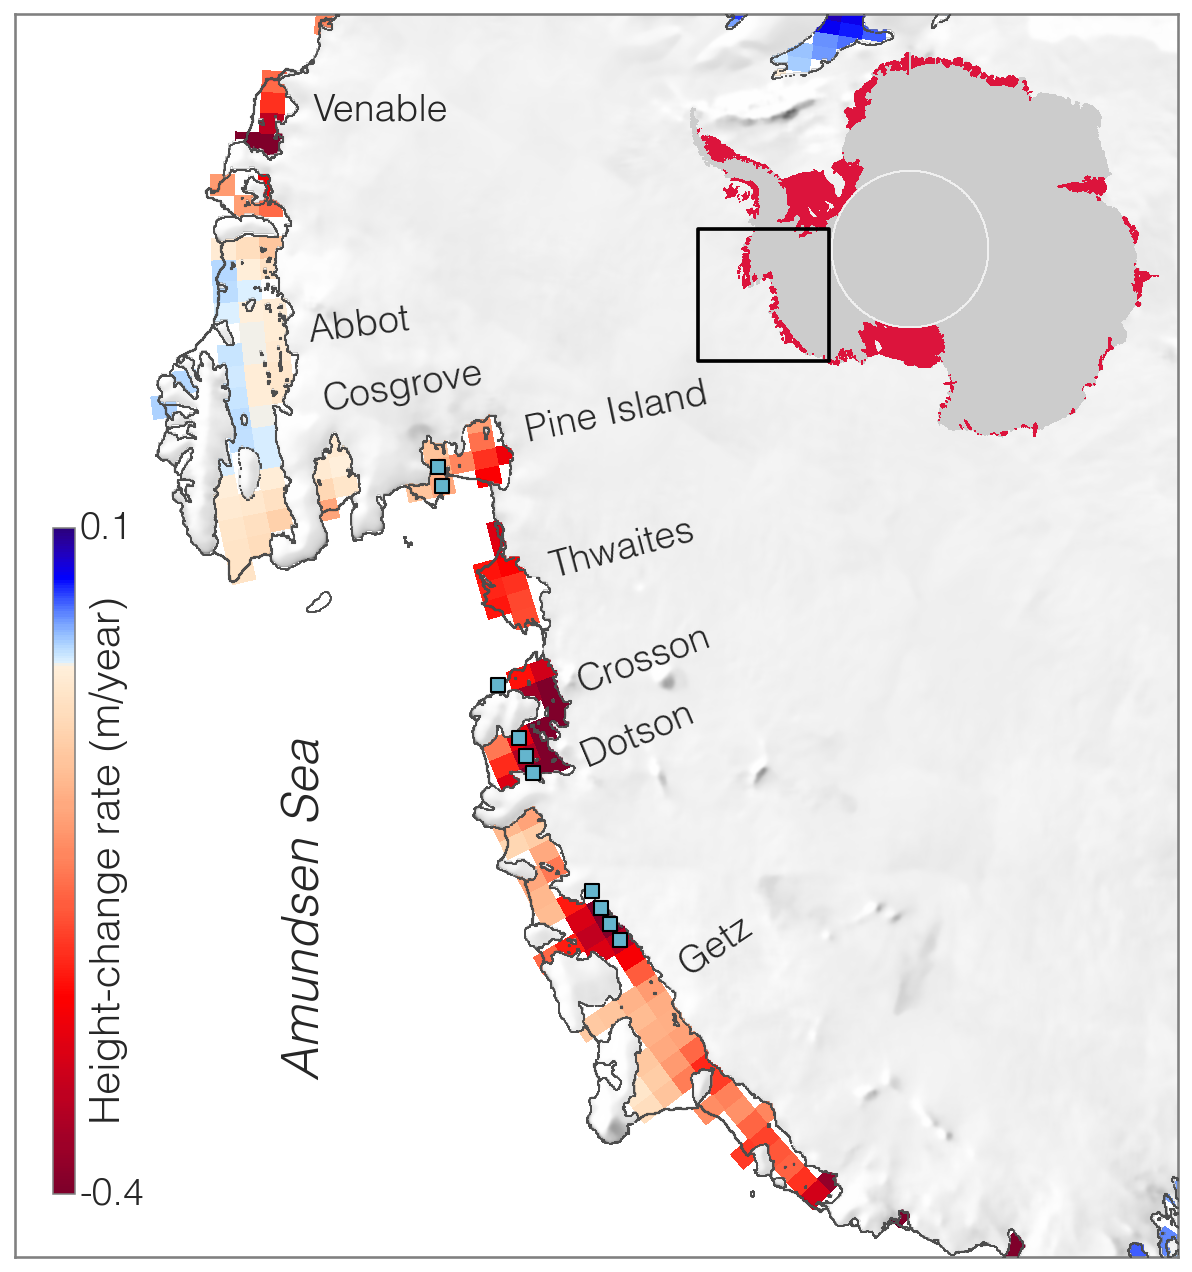
\includegraphics[width=.72\textwidth]{img/map_amundsen_v3.png}
  \caption[Map of Amundsen Sea (AS) ice shelves]{
  Amundsen Sea ice shelves in Antarctica. Map showing rate of change in surface-height (m/year) for the AS ice shelves. There are 140 30 km x 30 km grid cells in the region, and the colour represents the average $\del h/\del t$ for the period 1994--2012. Average height-change time series for each grid cell are analyzed in this chapter, and the ten blue squares show the locations of the time series used for stacking (see text).
  }
  \label{fig:map-amundsen}
\end{figure}


The ENSO phenomenon, a large-scale internal climate mode characterized by large changes of tropical sea-surface temperatures, is the strongest natural climate fluctuation at interannual time scales (Sup.~Fig.~\ref{fig:map-enso}). This sea-surface temperature anomaly is a response to changes in surface-air pressure (the Southern Oscillation) between the tropical eastern and the western Pacific Ocean waters, which reoccurs on average every four years \parencite{Latif2009, Philander1989}. Although some evidence of ENSO can be found in the Antarctic meteorological and ice-core records, a direct link between this tropical Pacific phenomenon and variations in the mass balance of the Antarctic Ice Sheet has yet to be demonstrated. Studies discussing this teleconnection present circumstantial evidence either based on a few sparse measurements with short time duration off the ice sheet/shelf \parencite[e.g.,][]{Dutrieux2014}, or an indirect assessment based on model experiments, ice cores and/or reanalysis products \parencite[e.g.,][]{Steig2013}. Here we present results from multivariate spectral analysis of fluctuations in ice-shelf height for the Amundsen Sea (AS), as a means of using direct observations to test the hypothesis that there is a connection between ENSO and Antarctic ice-shelf variability. We seek to quantify the extent to which tropical Pacific conditions may influence interannual changes in ice-shelf and ice-sheet mass balances.

\section{Methods}

\noindent
The 18-year record of changes in ice-shelf height presented by \textcite{Paolo2015, Paolo2015a} is the most comprehensive data set for studies of ice-shelf sensitivity to oceanic and atmospheric conditions available to date. Although more highly resolved in time ($\sim$3 months) and space ($\sim$30 km) in comparison with previous available data sets \parencite[e.g.,][]{Shepherd2010, Pritchard2012}, these time series still contain high noise levels, inherent to (a) the complex satellite radar altimeter measurement over ice surfaces \parencite{Paolo2015a, Davis1993, Arthern2001, Wingham2010, Remy2012} and (b) the wide range of time scales on which the ice shelves respond \parencite{Paolo2015a, Padman2003, Holland2015, Dutrieux2014}. In addition, the 18-year quarterly (3-month resolution) data is shorter and less well resolved in time compared with traditional climate records that typically span several decades at weekly/monthly resolution (see, for example, the NOAA Optimum Interpolation Sea Surface Temperature V2\footnote{\url{http://www.esrl.noaa.gov/psd/data/gridded/data.noaa.oisst.v2.html}}). Hence, the challenge lies in analyzing a set of short, noisy and potentially non-stationary\footnote{Stationarity means that statistical properties such as mean, variance and auto-correlation do not change with time.} time series.

We used the orthogonal-component decomposition of a time series known as Singular Spectrum Analysis \parencite[SSA;][]{Vautard1992, Golyandina2013, Elsner1996}. This technique has been applied extensively to the study of climate variability and other geophysical fields \parencite[][and references therein]{Ghil2002}; it was designed to handle the problem of describing cyclical behavior on short and noisy records, for which standard methods derived from Fourier analysis do not work well \parencite{Vautard1989, Ghil1991, Vautard1992, Groth2011}. The method is based on augmenting the original data set by constructing lagged versions of the original series (referred to as \emph{embedding}) with time delays of $1,...,M-1$, where $M$ is the length of the observation window (time scale under consideration). The augmented (or \emph{embedded}) data set can then be analyzed by standard Principal Component Analysis \parencite[PCA;][]{Jolliffe2002}.

In the multivariate case, where there is more than one time series, the same principle applies with the addition that the covariance matrix ($\vect C$) of the augmented data set (by embedding each series) includes cross-correlations, such that we can extract principal oscillations in time and space (common spectral properties). In particular, multivariate (or multichannel) SSA (MSSA) can separate distinct spectral components in a multivariate data set of limited length and in the presence of relatively high noise levels. The spectral decomposition by MSSA (Eq.~\ref{eigendecomposition}) yields a set of eigenvectors ($\vect e_k$, mode of oscillation) and a set of corresponding eigenvalues ($\lambda_k$, variance in the direction of the eigenvector). Provided that pairs of eigenvectors correspond to the same period ({\it oscillatory pairs}), they are the data-adaptive equivalent of sine-and-cosine pairs in Fourier  analysis: that is, they represent a temporal oscillation (phase-and-amplitude modulated in the case of MSSA; see Sup. material). The MSSA package used in this study also provides effective statistical tests to discriminate between potential oscillations from "white" noise (independent and identically distributed)---Monte-Carlo MSSA \parencite{Allen1996}. \textcite{Ghil2002} provide an overview and a comprehensive set of references to both the theory and applications of SSA and MSSA\footnote{Free software for implementation of SSA and MSSA, among other spectral techniques, is provided by the SSA-MTM Toolkit at \url{http://www.atmos.ucla.edu/tcd/ssa}}.

We used the Southern Oscillation Index (SOI) as a measure of ENSO, which is a standardized time series of observed sea-level pressure differences between Tahiti and Darwin, Australia. The SOI is one measure of the large-scale fluctuations in air pressure occurring between the western and eastern tropical Pacific during El Ni\~no and La Ni\~na episodes. The negative phase of the SOI represents below-normal air pressure at Tahiti and above-normal air pressure at Darwin. Prolonged periods of negative (positive) SOI values coincide with abnormally warm (cold) ocean waters across the eastern tropical Pacific typical of El Ni\~no (La Ni\~na) episodes (NOAA/NCDC\footnote{\url{https://www.ncdc.noaa.gov/teleconnections/enso/indicators/soi}}).

To analyze the data we first removed the trend of each ice-shelf time series separately, by using the time-domain Hodrick-Prescott filter \parencite{Hodrick1997} with the parameter value $\lambda= 1600$, as recommended by these authors for detrending quarterly data (Fig.~\ref{fig:series-decomposition} and Sup.~Eq.~\ref{hp-filter}). A trend-independent analysis is particularly important in the case of AS ice shelves where a strong (negative) trend dominates the height-change signal (Fig.~\ref{fig:series-decomposition}). Another reason for de-trending is that the trend varies (in some cases considerably) with location \parencite{Paolo2015, Pritchard2012, Shepherd2010}. Next, we normalized each residual time series by its standard deviation so that the variance equals one. We do this to avoid giving the variables (time series) with higher variances a greater weight in the analysis. Variables with the highest sample variances will tend to be emphasized in the first few principal components (our goal is to analyze common oscillatory behavior among the time series regardless of their ranges). Since both the ice-shelf time series and the SOI were standardized (centered and normalized) we focused the analysis on relative values. To further reduce the noise content in the initial data set, a common procedure is to pre-filter the original time series with standard PCA and retain the few leading components that explain larger portions of the total variance. MSSA is then applied to these leading principal components. We reduced the original set of 140 time series (see locations in Fig.~\ref{fig:map-amundsen}) to a set of 10 principal components (PCs) that explain over 47\% of the total variance of the de-trended data set (Sup.~Fig.~\ref{c4f10}).


\begin{figure}[!h]
  \centering
  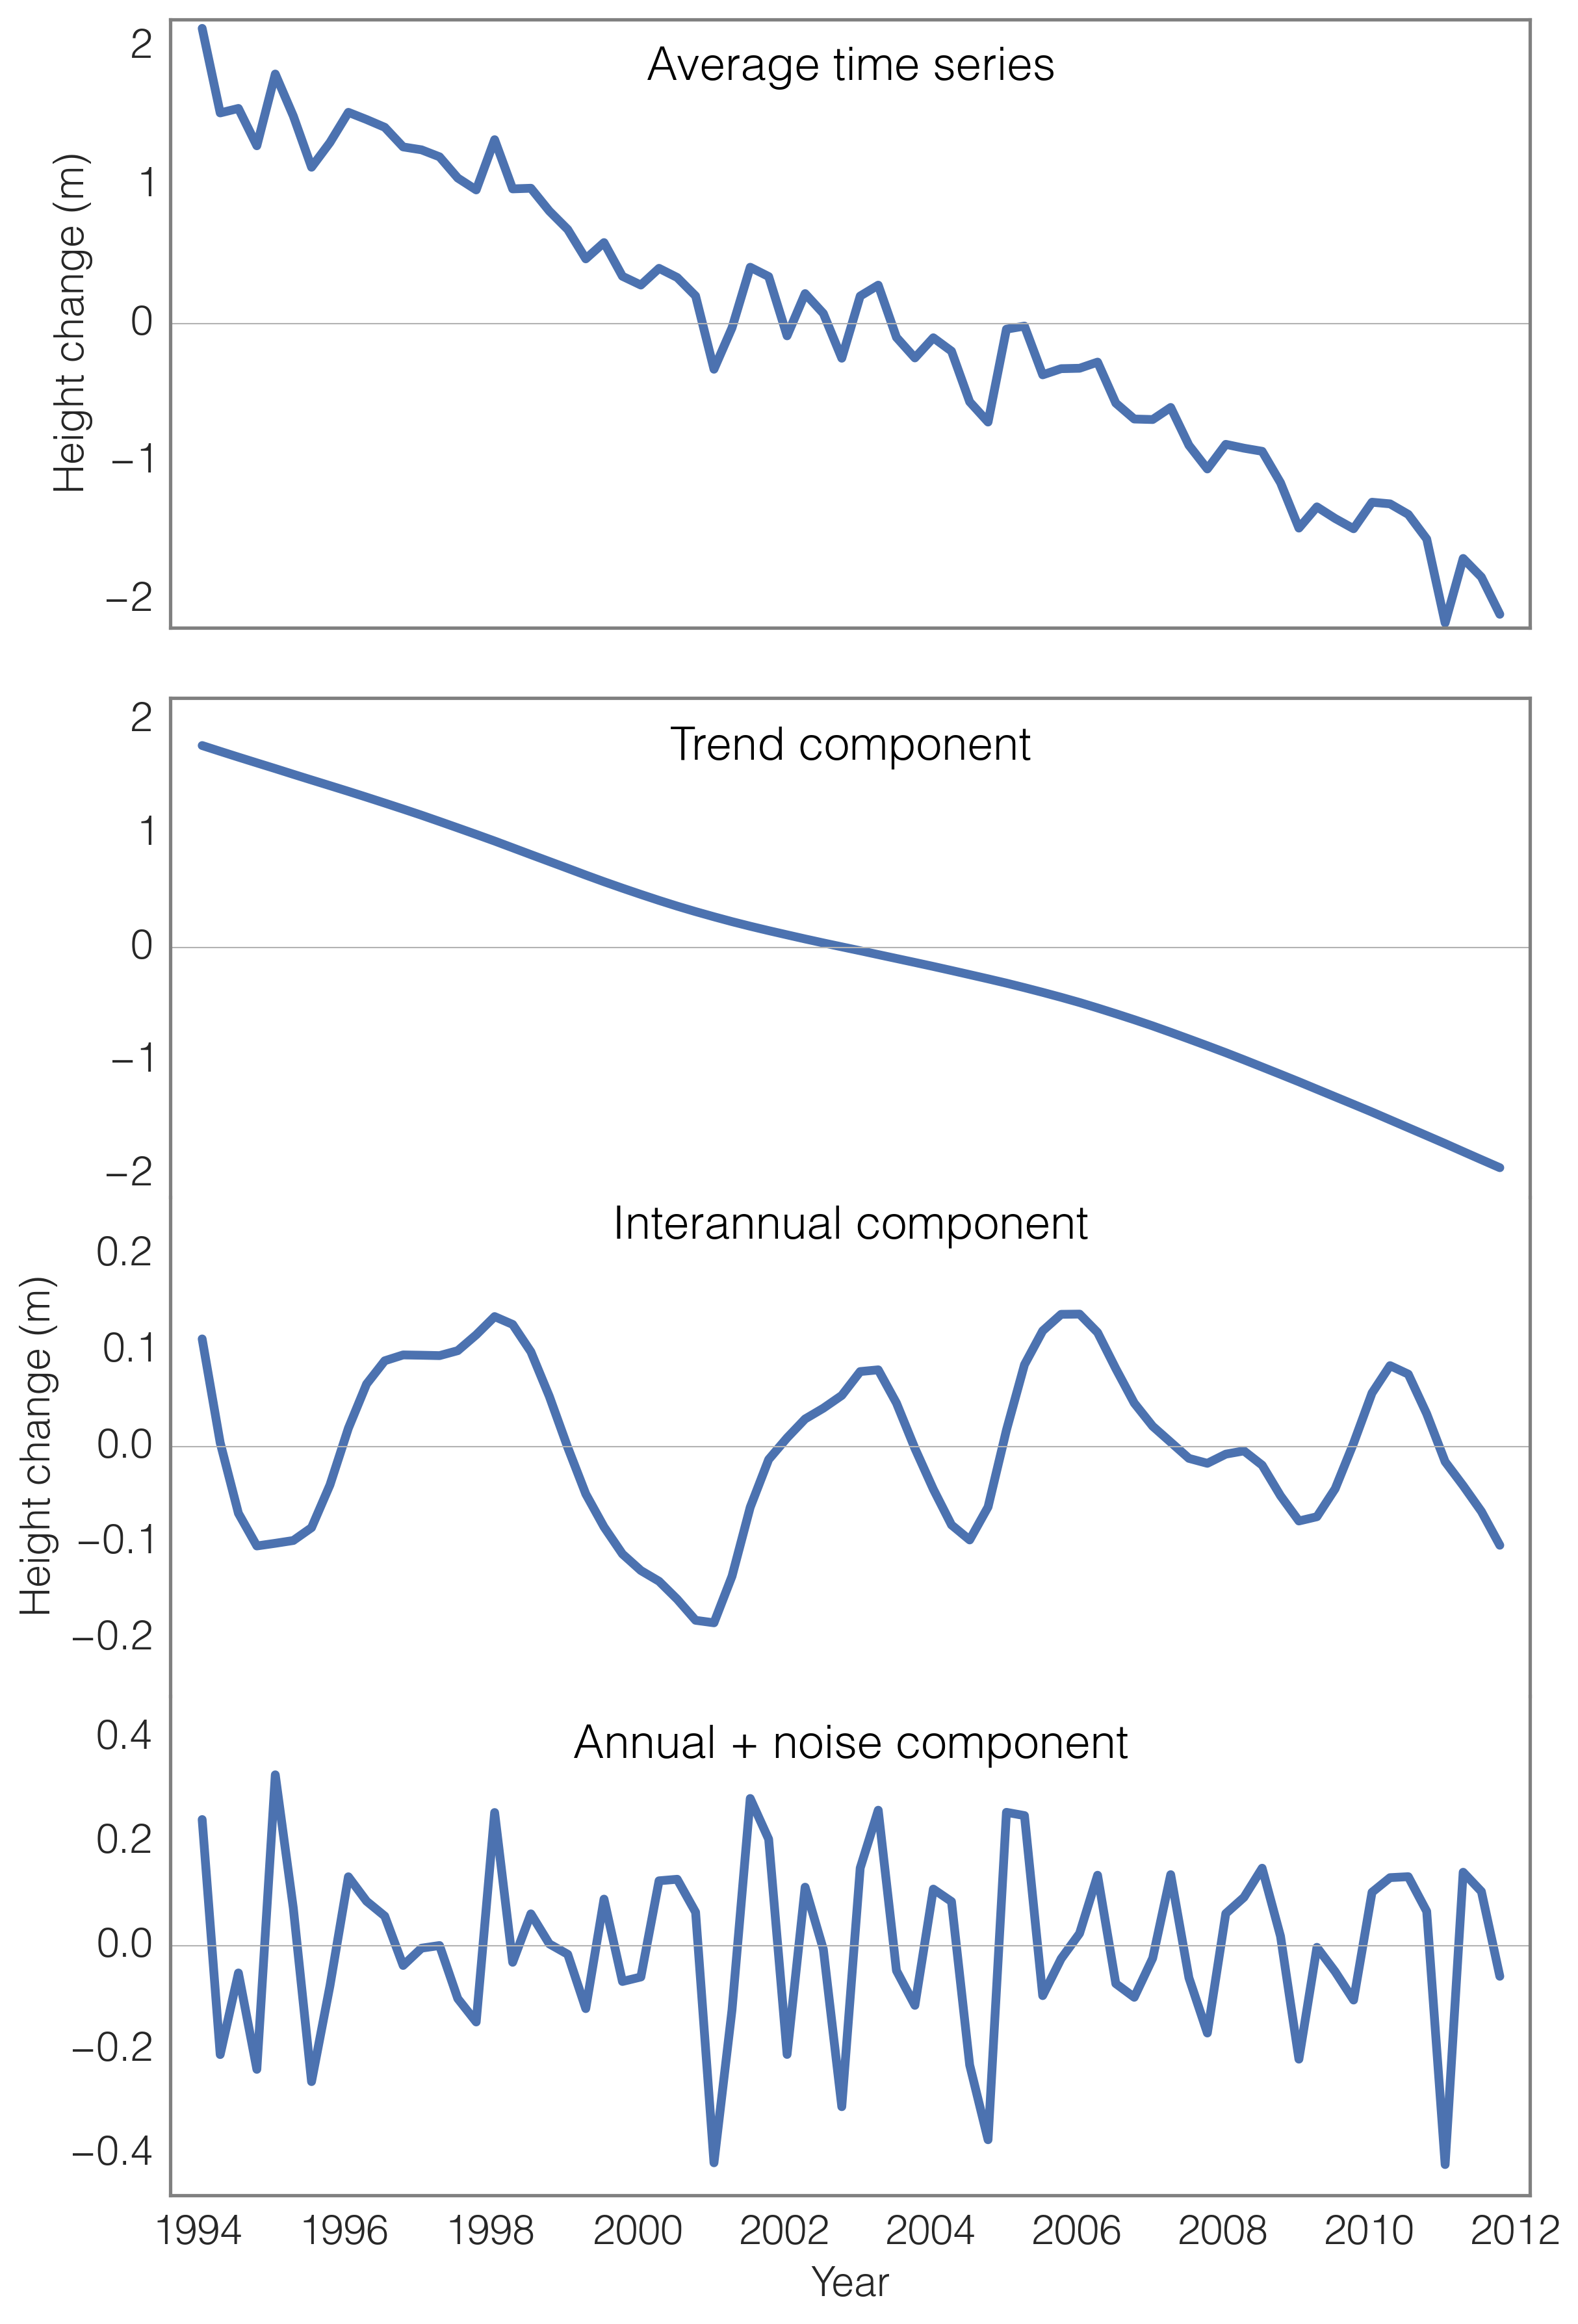
\includegraphics[width=.7\textwidth]{img/decompose_series_v2.png}
  \caption[Decomposition of AS ice-shelf height time-series]{
  Decomposition of AS ice-shelf height time series. (top panel) Average of all (140) time series of ice-shelf height changes in the Amundsen region. (bottom panel) Decomposition of the average time series into its trend, interannual, and annual-plus-noise components. The \textcite{Hodrick1997} filter was used to separate each component (see Supplementary material).
  }
  \label{fig:series-decomposition}
\end{figure}


The time scales under investigation are those characteristic of large-scale climate fluctuations at the interannual band. Therefore, our observation window ($M$) spans $\sim$9 years (sub-decadal). Since no spectral estimation should rely on any particular method, we extend our analysis with the (spectral-domain) multi-taper \parencite{Thomson1982} and maximum-entropy \parencite{Childers1978} methods (MTM and MEM, respectively) to estimate spectral content of reconstructed series (see below).


\section{Results and Discussion}

\noindent
In addition to the observed strong thinning trend in the AS ice shelves, there are relatively large fluctuations at both the interannual and annual time scales (Fig.~\ref{fig:series-decomposition}). Since an empirical `backscatter correction' has been applied to the height time series being analyzed \parencite{Paolo2015a}, we expect this correction to have removed much of the apparent seasonal signal that would have been observed in the uncorrected records (as an effect of fluctuations in backscatter due to changes in ice-shelf-surface properties). The same empirical correction also removes interannual signal that correlates with backscatter variations due to changes in surface state (rather than thickness). While we can explain (most of) the annual cycle by evoking the seasonal response of some ice-shelf-related mechanisms, such as surface accumulation, firn compaction, basal melting and changes in backscatter, we cannot yet directly attribute the interannual response to known interannual-scale climate processes. There are two reasons for this. First, there has been limited information, i.e., long-term and continuous observational records, on the ice-shelf state to allow inference of interannual variability \parencite{Paolo2015}. Second, the link between known interannual-scale climate processes and variations in thickness of the grounded ice sheet and floating ice is not quite clear from observations \parencite[e.g.,][]{Dutrieux2014, Steig2013, Turner2004}. 

When decomposing the standardized records of ice-shelf height into modes of oscillation (eigenvectors or EOFs) and looking at the variance explained by each eigenvector (Fig.~\ref{c4f3}), there is a clear separation between the first four EOFs (eigenvalues of rank 1--4) and the remaining eigenvectors. Arranging the same modes into power (equivalent to variance explained) versus the frequency that they represent, two facts become evident: 1) there is statistically-significant (90\% level) energy content in two particular bands---around 1 year and around 2.5--5 years; 2) MSSA is able to group in pairs EOFs for these particular frequency bands (eigenvalues of nearly-equal power representing the same frequency), indicative of an oscillatory behavior (Fig.~\ref{c4f3}). We note that none of the other EOFs (represented by their respective eigenvalues) are able to rise above the noise background. The three most energetic pairs of EOFs can then be used to decompose (or reconstruct) the original time series into two interannual components (RC 1--2 and RC 3--4), and one annual component (RC 5--6) (Fig.~\ref{c4f4}).


\begin{figure}[!h]
  \centering
  \vspace{1.4cm}
  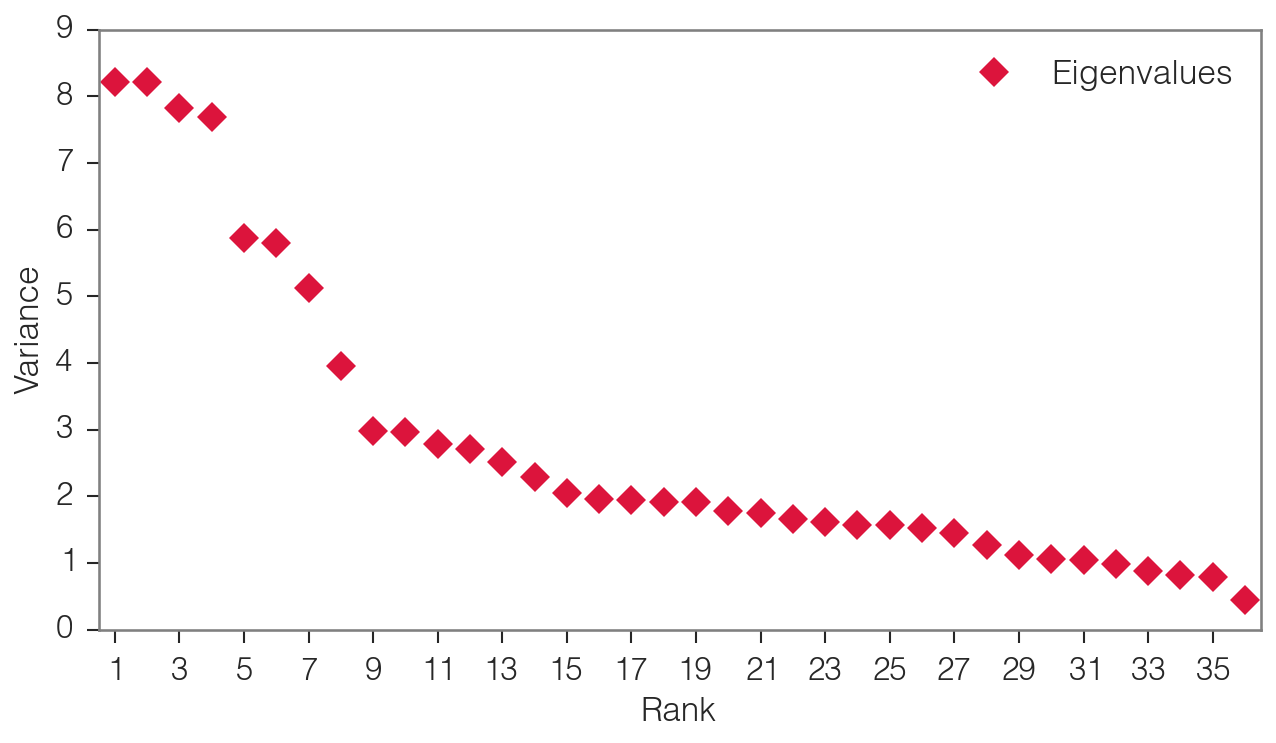
\includegraphics[width=.72\textwidth]{img/mssa_eigen_var_v3.png}\\
  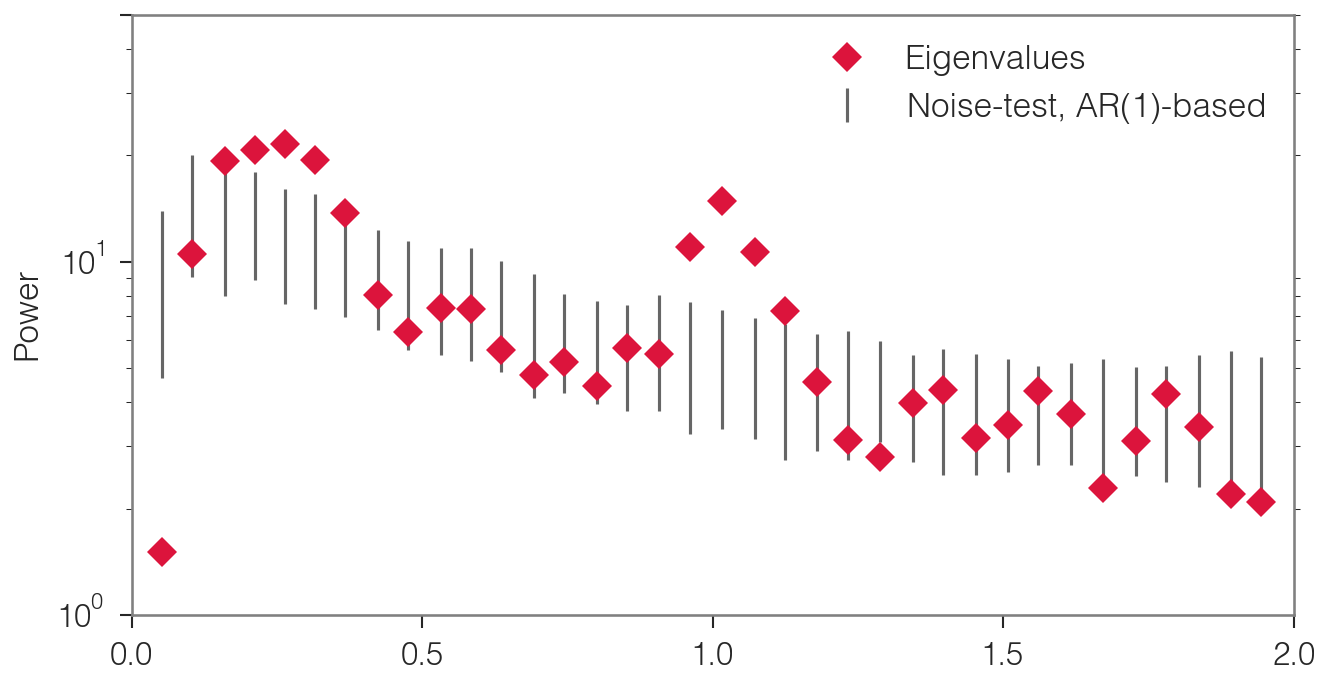
\includegraphics[width=.74\textwidth]{img/mssa_spec_ar1_v3.png}\\
  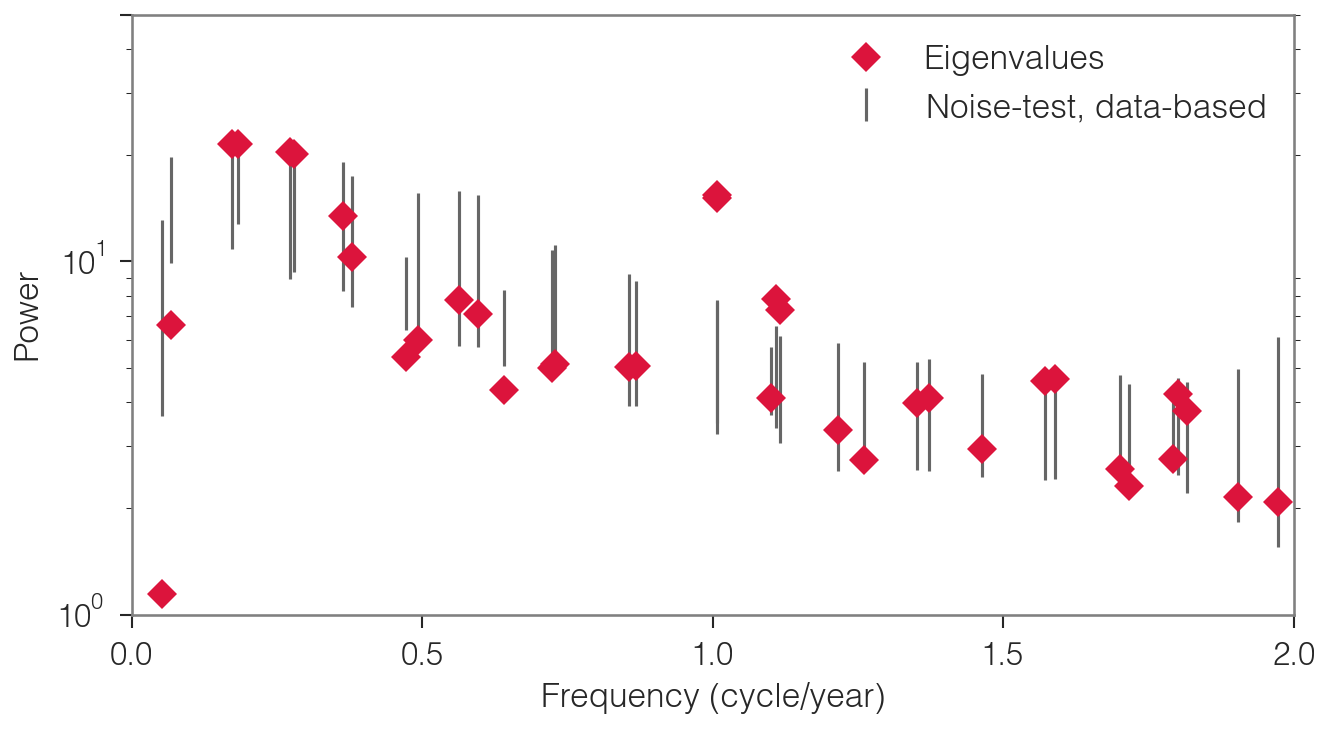
\includegraphics[width=.74\textwidth]{img/mssa_spec_data_v3.png}
  \vspace{1.4cm}
\end{figure}
%\clearpage
\begin{figure}
  \captionsetup{labelformat=adja-page}
  %\ContinuedFloat
  \caption[Singular spectrum of AS ice-shelve height time-series]{
  Singular spectrum of AS ice-shelve height time series. The `diamonds' represent the eigenvalues of the auto-correlation matrix $\vect{C}^{(M)}$ (Eq.~\ref{eigendecomposition}). The vertical bars are 90\% confidence intervals for 100 red-noise realizations with the same variance and decorrelation time as the original series. The values that stand out above the error bars are statistically significant. (top) Variance vs. eigenvalue rank. (middle) Eigenvalue vs. dominant frequency of corresponding eigenvector, using an AR(1) model as basis (the frequencies are well defined). (bottom) Eigenvalue vs. dominant frequency using the data as basis, where the frequency of each eigenvector is obtained by least-square fitting the corresponding EOF to a sine function (the frequencies are approximated). Note that eigenvalues 1--4 (the interannual components) appear well separated from the remaining 5--36 (the seasonal-plus-noise components). The spectra were produce with Monte-Carlo MSSA using window width (number of lags) $M=36$ ($\sim$9 years).
  }
  \label{c4f3}
\end{figure}
%\clearpage


\begin{figure}[!h]
  \centering
  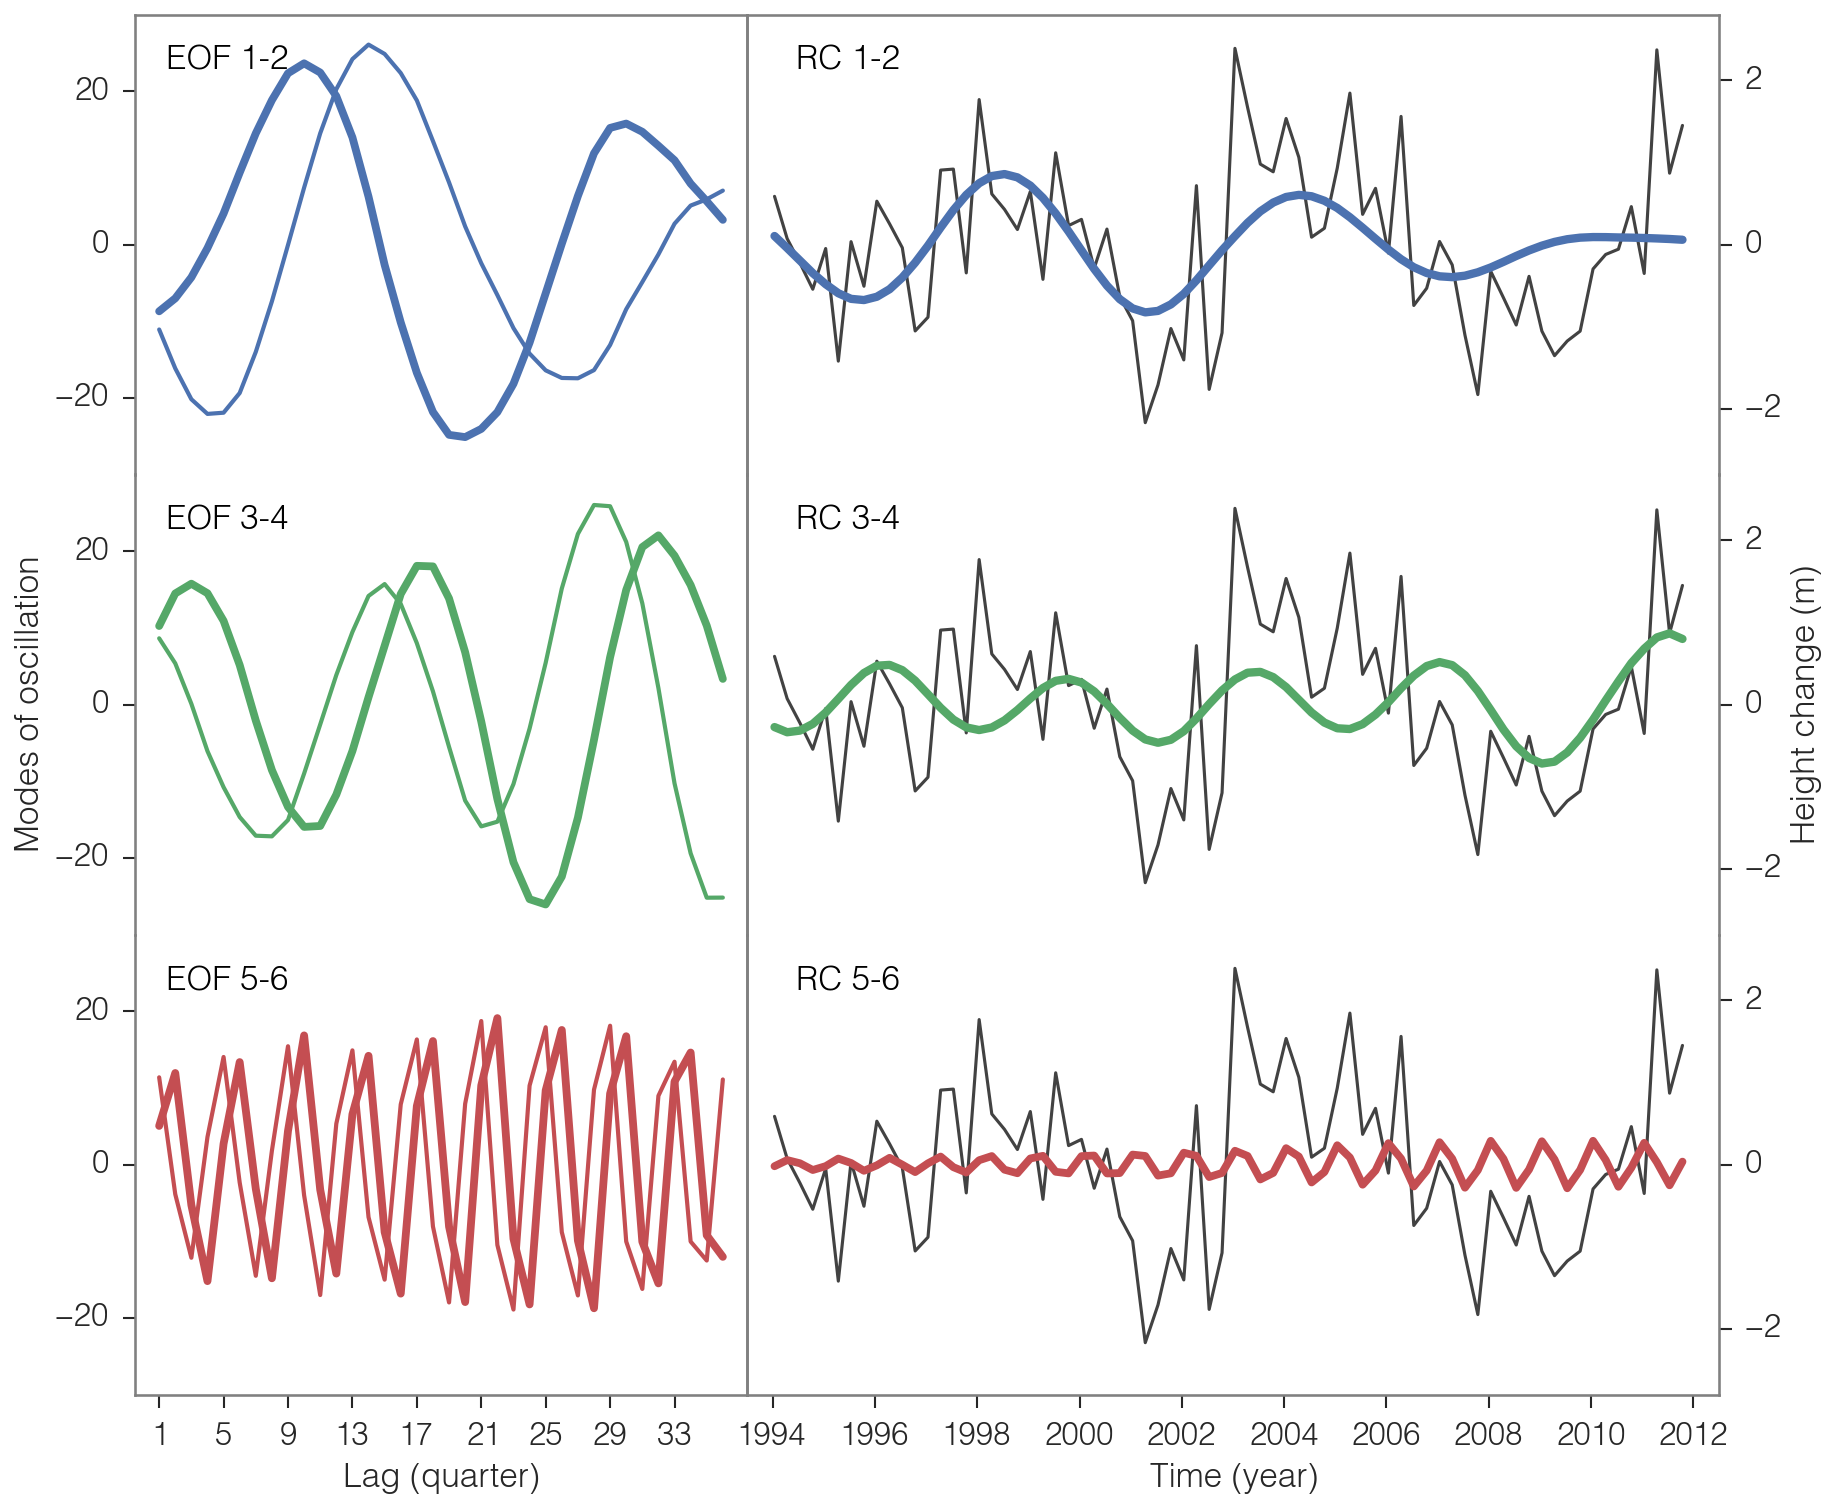
\includegraphics[width=\textwidth]{img/mssa_eof_rc_v2.png}
  \caption[Modes of oscillation in the ice-shelf height time-series]{
  Modes of oscillation in the ice-shelf height RA time series. (left) The MSSA empirical orthogonal functions paired as EOFs 1--2, 3--4 (interannual components) and 5--6 (annual component). Note the phase quadrature ($\sim$$\pi/4$ shift) between pairs, indicative of a temporal oscillation. (right) The reconstruction of each pair of modes in the time domain. This is equivalent to filtering the original time series (in gray) with respect to particular frequencies (periodicities). The reconstruction was done for each of the 140 individual grid-cell time series from the original RA-derived data set (this is one time series as example; see Fig.~\ref{fig:rc1234-all}).
  }
  \label{c4f4}
\end{figure}


Similarly, using all the significant components together (EOFs 1--2, 3--4 and 5--6) we reconstructed the ice-shelf height record (RC 1--6; Fig.~\ref{c4f5}), such that (a) we filtered out from the original time series all uncorrelated signals and measurement noise, and (b) we were able to estimate the power spectrum of the (significant) interannual and annual components (Fig.~\ref{c4f5}). Although we are particularly interested in identifying interannual fluctuations, we opted to retain the annual component in the reconstruction. This serves as a control for the MSSA procedure; since we know that ice shelves respond at the seasonal scale (e.g., precipitation-driven surface mass balance), we expect that this signal should be clearly detectable in our analysis. The MEM power spectrum of the reconstructed time series (Fig.~\ref{c4f5}) shows three peaks at frequencies $\sim$0.2, $\sim$0.3 and $\sim$1.0 cycles/year ($\sim$5, 3 and 1 years, respectively). The MTM spectrum (Fig.~\ref{c4f5}) shows significant (95\%) spectral peaks at frequencies 0.20--0.23 and 1.0 cycles/year ($\sim$5--4.3 and 1 years, respectively). While the MEM approach is optimal when applied with low-resolution (low-order autoregression) to denoised series (reconstructed components), producing a smooth curve where only well-defined peaks "survive" \parencite{Penland1991}, the MTM spectrum offers a good trade-off between high spectral resolution and statistical confidence levels that are independent of the spectral power \parencite{Mann1996, Percival1993}. In addition, the MTM implemented here \parencite{Mann1996} makes use of a "robust" estimate of the background noise, and performs a harmonic test.


\begin{figure}[!ht]
  \centering
  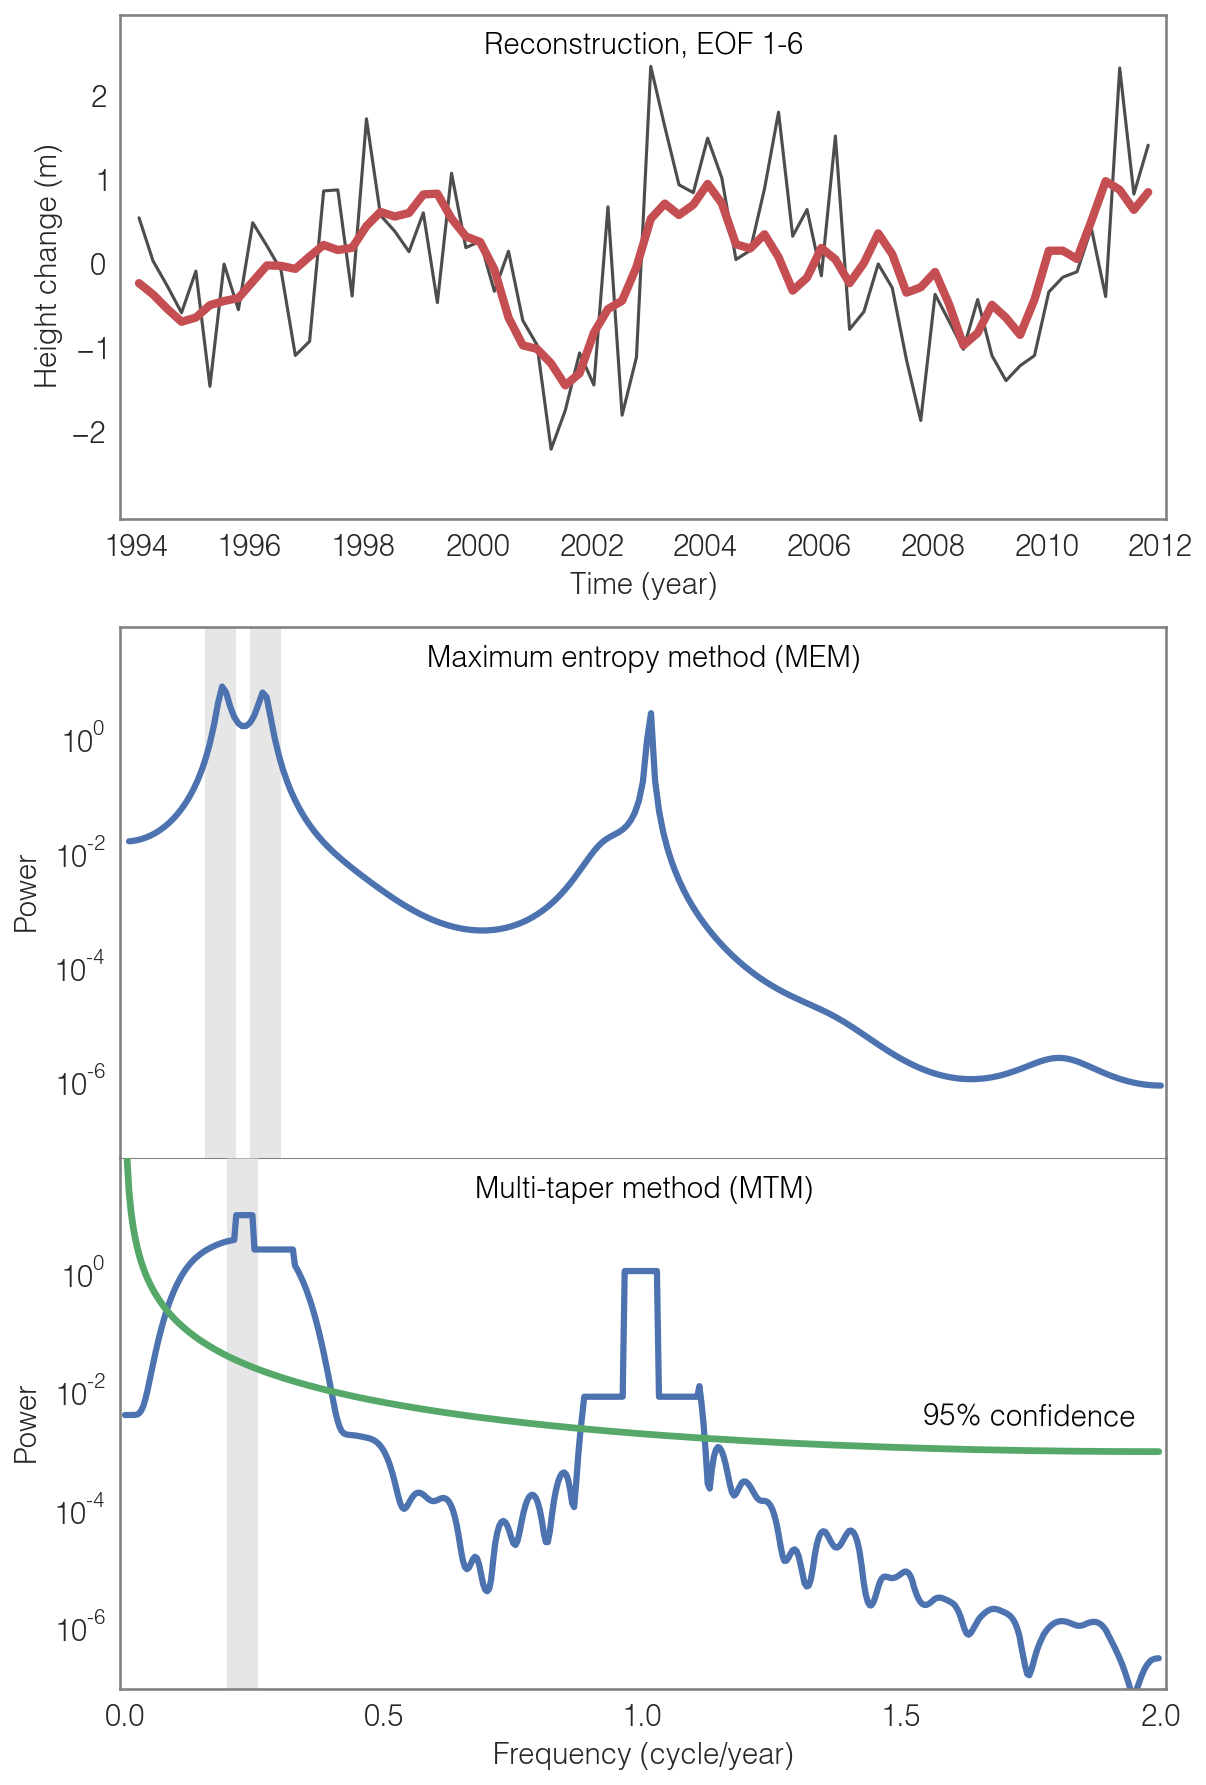
\includegraphics[width=.72\textwidth]{img/mem_mtm_amu_v2.png}
  \caption[Power spectrum of ice-shelf height reconstructions]{
  Power spectrum of the reconstructed RA-derived ice-shelf height time series. (top) Reconstruction of ice-shelf surface height series using the three leading pairs of EOFs (1--2, 3--4 and 5--6). (bottom) Power spectra by the maximum entropy and multi-taper methods (MEM and MTM, respectively). While the MEM spectrum is smooth (order 20) and focuses on the dominant frequencies, the MTM offers higher spectral resolution and confidence level of the estimated spectrum. The regular-shaped peaks represent the frequencies that passed a harmonic test, included in the MTM package. The gray stripes demarcate the dominant frequencies at the interannual band detected by each spectrum (0.18 and 0.26 cycle/year for MEM, 0.22 cycle/year for MTM).
  }
  \label{c4f5}
\end{figure}


To obtain the ENSO signal we reproduced the analysis performed by \textcite{Ghil2002} (univariate SSA) on the SOI time series, using an updated version of the index (from NOAA\footnote{\url{https://www.ncdc.noaa.gov/teleconnections/enso/indicators/soi/}}) spanning the period 1951 to 2015. The SSA spectrum of the SOI series (Fig.~\ref{c4f6}) clearly identifies two significant pairs of eigenvectors, which have been attributed to the low-frequency (4--5 years) and quasi-biennial ($\sim$2.5 years) modes of ENSO \parencite[e.g.,][]{Ghil2002, Philander1989} (Fig.~\ref{c4f6}). We then reconstructed the SOI series using these two modes (RC 1--4; Fig.~\ref{c4f7}), and applied the MEM and MTM in the same way as done for the ice-shelf time-series reconstruction (Fig.~\ref{c4f8}). 


\begin{figure}[!ht]
  \centering
  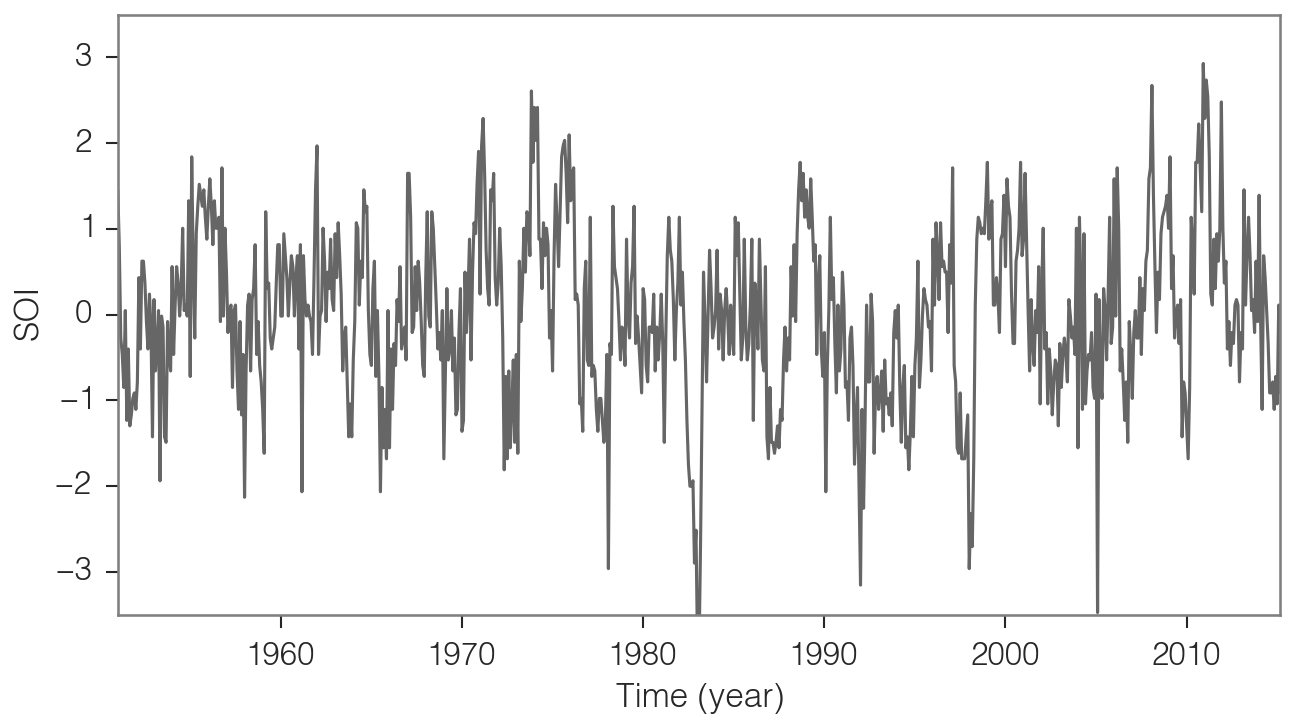
\includegraphics[width=.72\textwidth]{img/soi_time_series.png}\\
  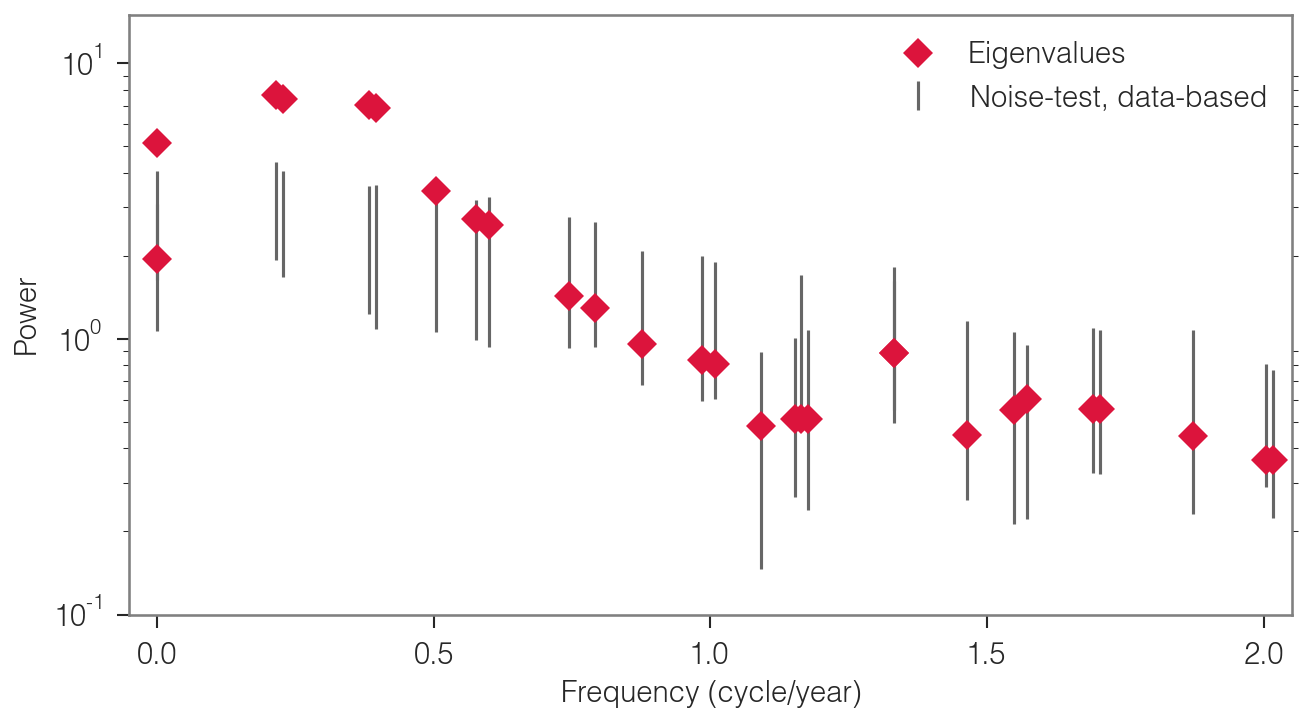
\includegraphics[width=.72\textwidth]{img/ssa_spec_soi.png}
  \caption[Singular spectrum of the SOI time-series]{
  Singular spectrum of the SOI time series. (top) SOI time series from NOAA (1951--2015). (bottom) Singular spectrum analysis of the SOI time series ($M = 76$, $\sim$6.3 years). The vertical bars are 90\% confidence intervals for 100 red-noise realizations.
  }
  \label{c4f6}
\end{figure}


\begin{figure}[!ht]
  \centering
  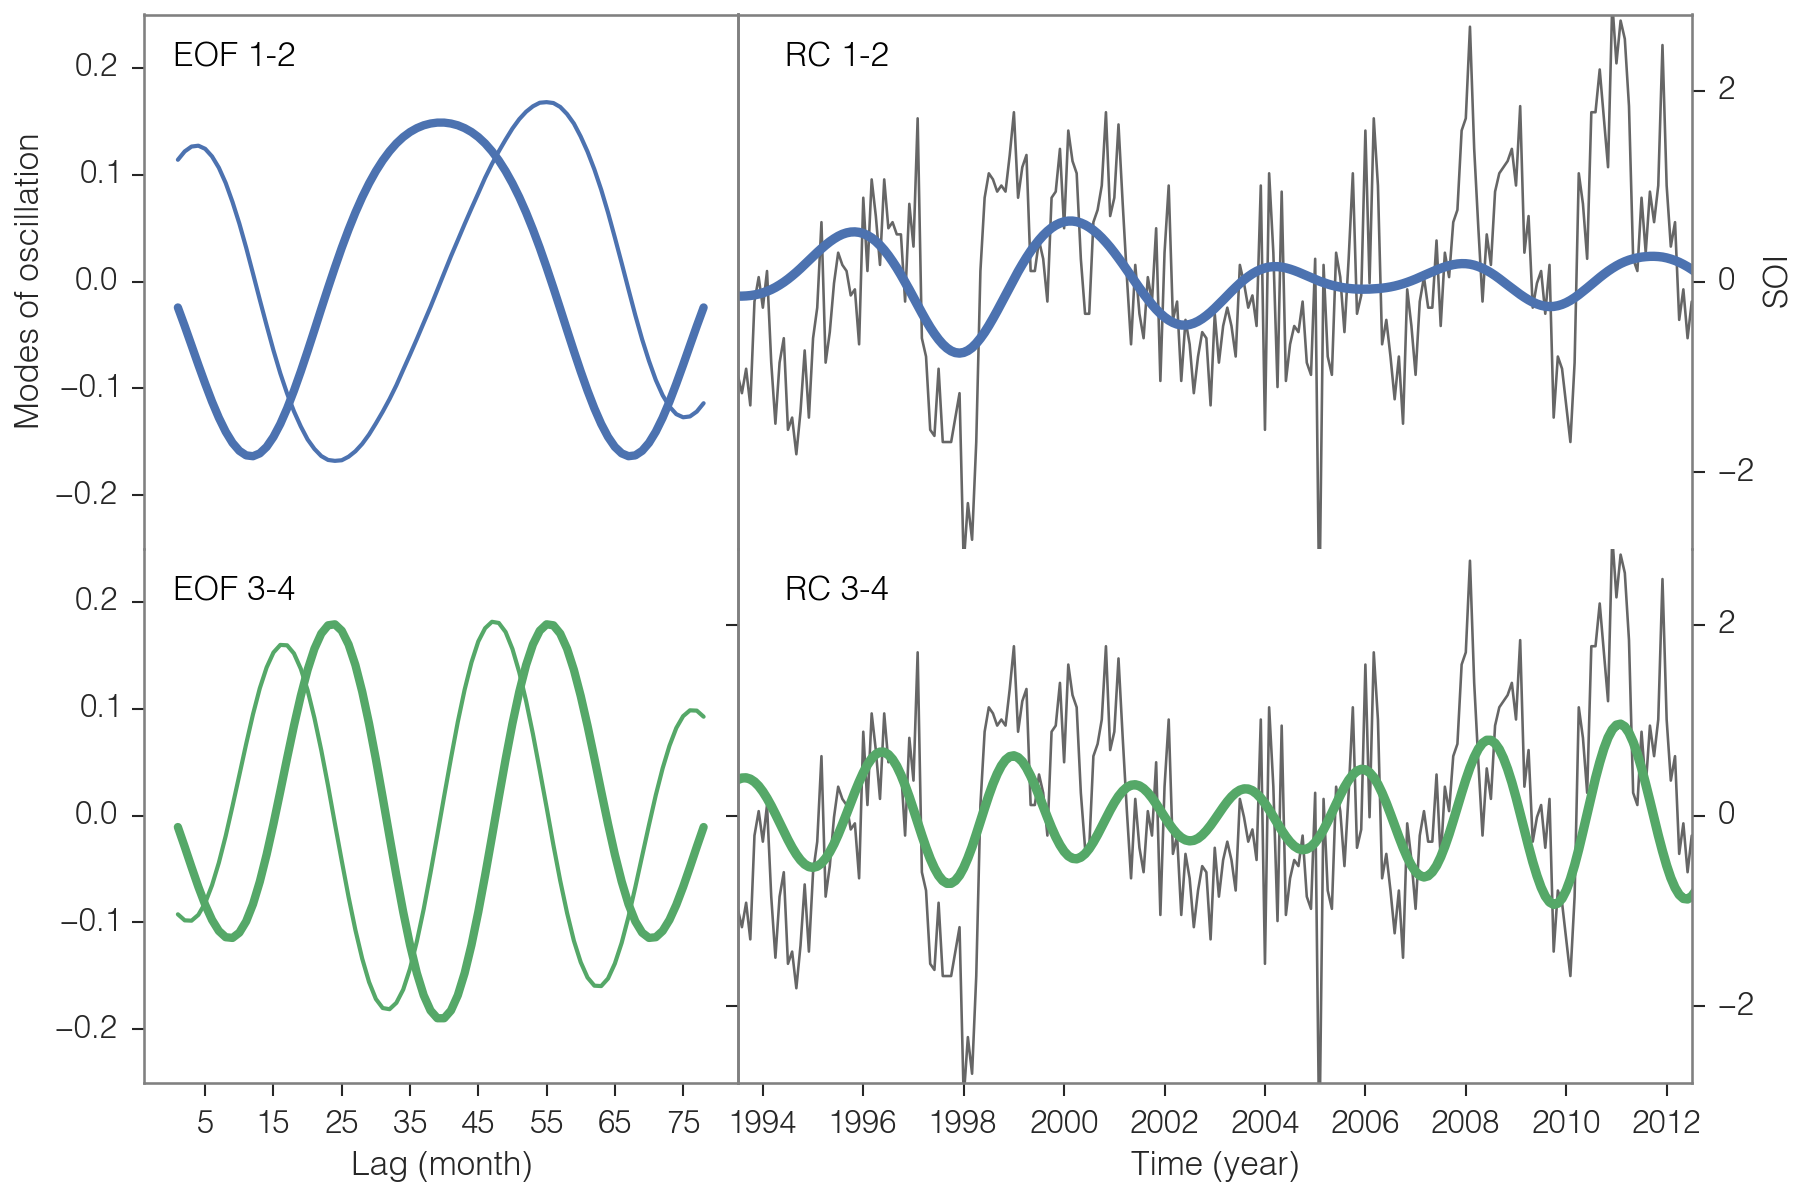
\includegraphics[width=\textwidth]{img/ssa_eof_rc_v3.png}
  \caption[Modes of oscillation in the SOI time-series]{
  Modes of oscillation in the SOI time series. (left) Leading pairs of EOFs (1--2 and 3--4). (right) Reconstructions of the SOI series using the respective EOFs, corresponding to the low-frequency (blue) and quasi-biennial (green) modes of ENSO. In the background is the original SOI series.
  }
  \label{c4f7}
\end{figure}


\begin{figure}[!ht]
  \centering
  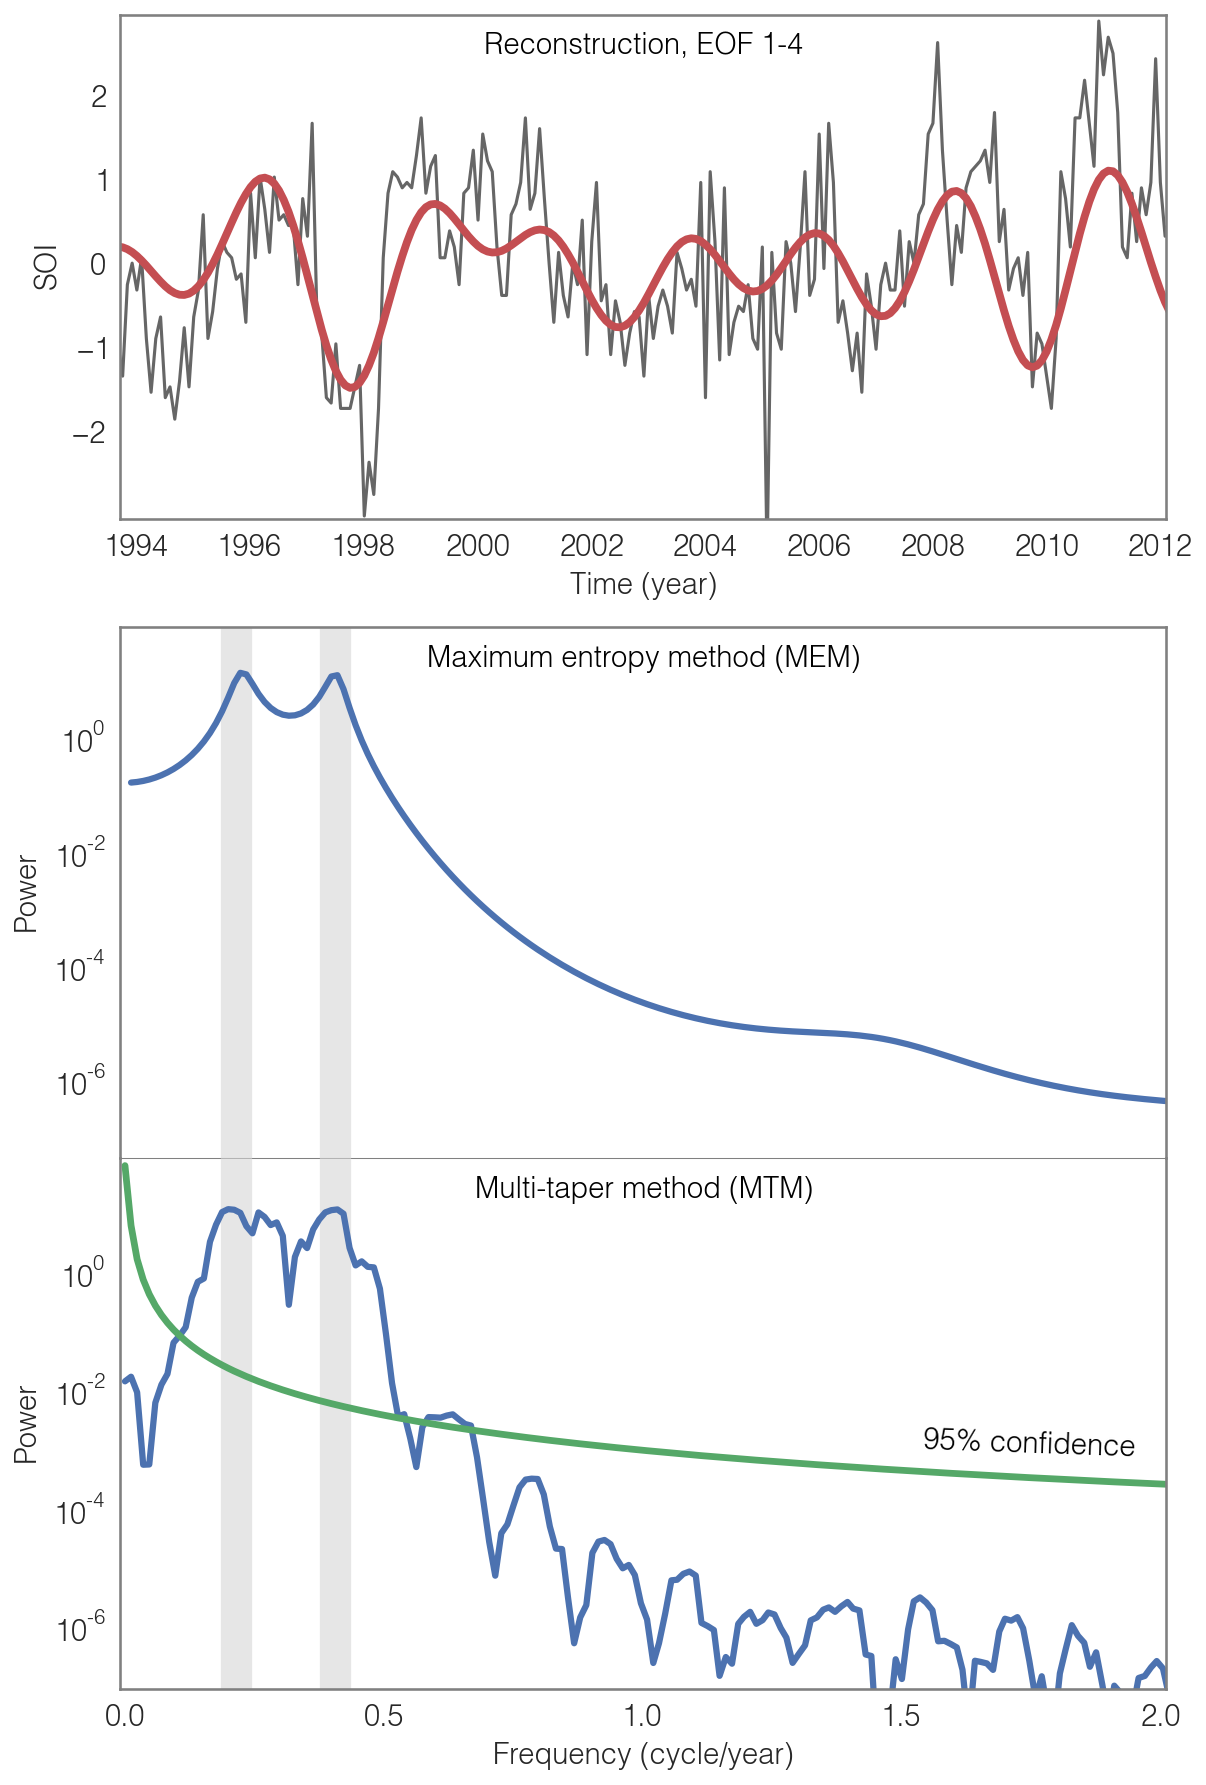
\includegraphics[width=.72\textwidth]{img/mem_mtm_soi_v2.png}
  \caption[Power spectrum of the SOI reconstruction]{
  Power spectrum of the reconstructed SOI time series. (top) Reconstruction of SOI series using the two leading pairs of EOFs (1--2 and 3--4). (bottom) Power spectra by the maximum entropy and multi-taper methods (MEM and MTM, respectively). The gray stripes demarcate the dominant frequencies at the interannual band detected by each spectrum, which in this case are the same (0.21--0.22 and 0.40--0.41 cycle/year, or $\sim$4.5 and $\sim$2.5 years, respectively).
  }
  \label{c4f8}
\end{figure}


The spectra of both reconstructions (ice-shelves height and SOI) show most of the energy in the frequency band of $\sim$0.2--0.4 (2.5--5) cycle/year (years). While the MEM spectrum appears to identify two distinct oscillations (double peak; Fig.~\ref{c4f5}) the MTM is not able to distinguish between these two components in the ice-shelf signal. Instead, the MTM shows significant (95\%) spectral energy in one dominant frequency ($\sim$4.5 years).

We reconstructed all 140 individual grid-cell time series (the RA data) using the two leading pairs of EOFs (RC 1--4; Sup. Fig.~\ref{fig:rc1234-all}). Since there is substantial coherent information within the RCs, we selected 10 of these reconstructions that display high amplitude and coherence (locations are shown in Fig.~\ref{fig:map-amundsen} and time series 40--49 are shown in Sup. Fig.~\ref{fig:rc1234-all}) and stacked them in order to smooth out incoherent signal and enhance common fluctuations. To facilitate visual comparison, we multiplied the SOI RC 1--2 (the low-frequency mode of ENSO) by $-1$ (i.e., flipped the series upside-down), such that positive (negative) anomalies now represent El Ni\~no (La Ni\~na) events. We also centered and normalized both the ice-shelf height and SOI reconstructions.

The result reveals a strong correlation between the interannual signal for these 10 stacked ice-shelf-height reconstructions and the low-frequency mode of ENSO (the SOI reconstruction; Fig.~\ref{c4f9}). This implies that in the AS time-series decomposition by MSSA the two leading pairs of EOFs (eigenvectors 1--2 and 3--4) are, in fact, describing one dominant mode of variability (RC 1--4), an oscillation in the same frequency band as the $\sim$4.5-year-mode of ENSO. The two reconstructions (ice-shelf height and SOI) show phase coherence and remarkable agreement in their amplitude modulation (peak-to-peak amplitude difference in the standardized series).

The apparent shift between the two time series is 2--6 months, with the height record lagging the (inverse) SOI. The positive correlation between the reconstructed ice-shelf height and inverse of the SOI reconstruction implies that there is a direct relationship between El Ni\~no events and height increase in the AS ice shelves. The expected lag is complicated by the multiple processes and complex pathways by which the atmospheric changes in the Amundsen Sea influence the ice-shelf thickness. There is, also, some uncertainty in the exact lag, given that the ice-shelf time series have lower resolution (quarterly) relative to the monthly values of SOI, and that the distribution of height measurements within each 3-month interval is heterogeneous \parencite{Paolo2015a}. 


\begin{figure}[!ht]
  \centering
  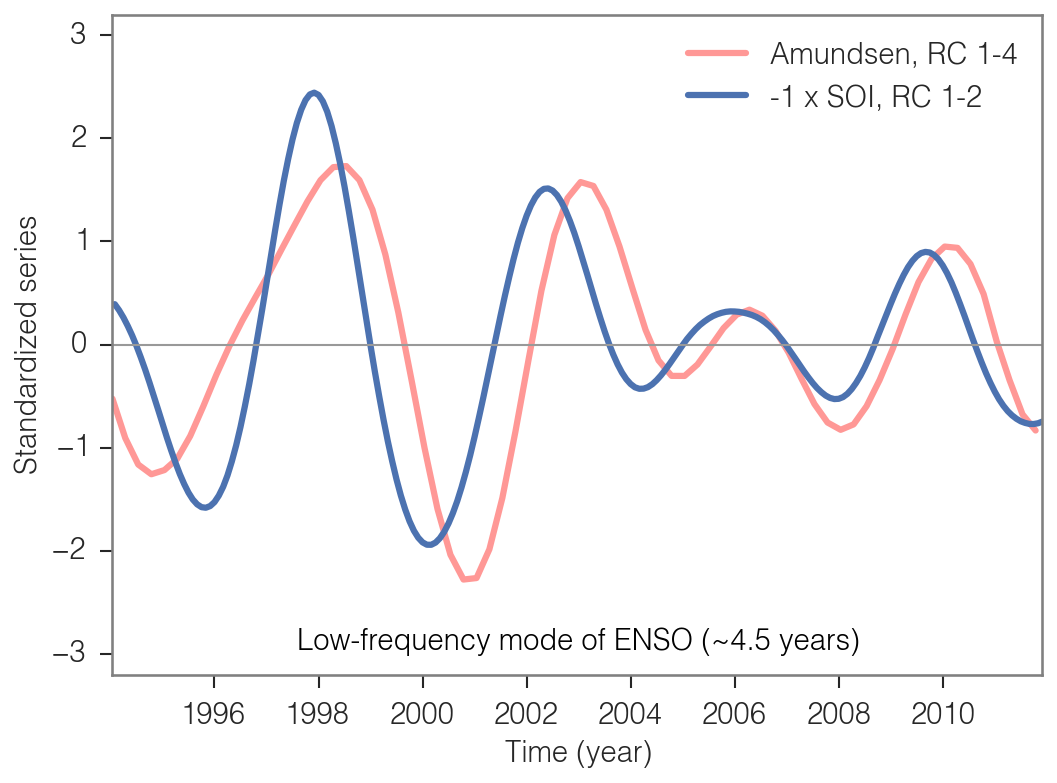
\includegraphics[width=.72\textwidth]{img/amu_soi_modes.png}
  \caption[Dominant mode of interannual variability (10 RCs)]{
  Dominant mode of interannual variability. Reconstruction of the dominant mode of interannual variability for the AS ice-shelf height and the SOI. Both series show the same dominant frequency of 0.20--0.23 cycle/year (periodicity of $\sim$4.5 years), which corresponds to the low-frequency mode of ENSO.
  }
  \label{c4f9}
\end{figure}


Future analyses of these time series will consider the different mechanisms by which atmospheric variability, including the strong ENSO signal, can affect ice-shelf thickness and height. Here, we consider just one mechanism, the changing surface mass flux from snowfall.

The majority of precipitation in Antarctica comes from synoptic-scale\footnote{Synoptic scale, or cyclonic scale, is the horizontal scale typical of mid-latitude atmospheric depressions (e.g., extra-tropical cyclones); spatial scale on the order of 1000 km.} storms (cyclones), which are most intense in winter. These cyclones form in mid-latitude ocean basins and, as they mature and intensify, they move southeast, picking up moisture from the surrounding seas. The influence of these cyclones is substantial along the Antarctic coast, particularly in West Antarctica where relatively low ice-sheet elevations permit easier transit of storms \parencite{Riffenburgh2007}. As they move inland where temperatures are colder, the moisture freezes leading to heavy snowfalls. Cyclonic activity fluctuates interannually in association with climatic teleconnections such as ENSO, particularly in the Pacific sector of West Antarctica (see Sup.~Fig.~\ref{fig:map-enso}). Cyclonic activity tends to increase (decrease) on the western side of the Antarctic Peninsula during El Ni\~no (La Ni\~na) events \parencite{Riffenburgh2007}. Consistent with these dynamics, \textcite{Kwok2002} found that surface temperatures over the eastern Bellingshausen Sea were positively correlated with the SOI, that is, temperatures were colder than normal during El Ni\~no events. Cullather et al. (1996) showed that nearly 40\% of the moisture flux into Antarctica occurred along the West Antarctic coast, where the precipitation variability correlated well with ENSO---with more (less) moisture convergence during El Ni\~no (La Ni\~na/normal) events. A strong positive correlation between ENSO and precipitation in the Amundsen Sea region was also found by \textcite{Genthon2003}. The strongest correlations associated with the ENSO signal, however, appear to occur with the sea-ice extent anomaly in the Amundsen and Bellingshausen seas, where El Ni\~no events generate a corresponding signal (decrease) in the ice extent ~6 months later \parencite{Yuan2000, Turner2004}.

The correlation between the inverse of SOI and RA-derived ice-shelf height is broadly consistent with this view of changing moisture transport for differing ENSO states. Ice-shelf heights are highest following the peak of an El Ni\~no event (warmer ocean surface in the tropical Pacific) during which we expect higher-than-average precipitation over the ice shelves and coastal regions of the grounded ice sheet. More work is required, however, to determine whether the measured interannual changes in ice-shelf height are consistent with the estimated change in surface mass balance between El Ni\~no events and neutral or La Ni\~na conditions. Furthermore, there is strong circumstantial evidence that some of the interannual variability in ice-shelf height is due to changing basal-melt rate as inflows of CDW under the AS ice shelves change, possibly due in part to variations in thermocline\footnote{ The thermocline is the transition layer between the mixed layer at the surface and the deep water layer. The definitions of these layers are based on temperature. The mixed layer is near the surface where the temperature is approximately that of surface water.} height \parencite{Dutrieux2014}. The CDW inflow and thermocline depth are both dependent on changes in the wind field, and so are expected to be correlated with the atmospheric changes influencing ice-shelf surface-mass balance.

Although the ENSO signal is clearly identified in our analysis, we emphasize that, over 18 years, the long-term trend actually overwhelms the interannual fluctuation in the AS ice-shelf height change signal by 1--2 orders of magnitude. On short periods of one to a few years, however, the rate of change of ice-shelf height ($\del h/\del t$) can vary about the trend by more than 50\%, implying that height trends based on short satellite records and limited-duration field campaigns might also be in error by this amount. We note that the amplitude of the interannual variation, while explaining a larger portion of the total variance, is comparable to that of the seasonal-plus-noise fluctuation. 


\section{Conclusions}

\noindent
We have presented a signal-detection procedure that (a) optimizes the fundamental signal-to-noise ratio problem through the combination of multivariate singular spectrum analysis, principal component analysis, maximum entropy and multi-taper methods; and (b) tests assumptions regarding the detectability of signals immersed in background noise, which is of fundamental importance in analyzing short and noisy records. We have shown that there is significant variability in ice-shelf height in the AS sector, particularly at the interannual scale. This interannual response is strongly correlated with the low-frequency mode of El Ni\~no-Southern Oscillation. Due to the convoluted nature of different modes of variability and lack of observations, an ENSO signature in Antarctica has been suggested but not unequivocally demonstrated so far. Thus, our results are the first direct observational evidence of a teleconnection between climate dynamics in the tropical Pacific Ocean and the mass balance of Antarctic ice shelves and, through the buttressing effect, the Antarctic Ice Sheet. This may ultimately allow us to improve our models for predicting future ice loss.


\section{Supplementary material}

\subsubsection*{Singular Spectrum Analysis}

\noindent
SSA is essentially an application of the Karhunen-Lo\`eve spectral decomposition theorem in the time domain \parencite[][, and references therein]{Ghil2002}. The particular strength of SSA is that the basis functions in terms of which the data are decomposed, are determined from the time series itself (unlike the predefined orthonormal sine and cosine bases as in the Fourier analysis \parencite{Blackman1958}). The basic assumption is that the information contained in a \emph{continuous} variable and its first-to-($M - 1$)th derivatives can be approximated by a \emph{discrete} time series and lagged copies of itself, by $1,...,M - 1$ time steps \parencite[][chap. 4]{Elsner1996}. The multivariate version of SSA (MSSA) is an advanced data-adaptive method to analyze oscillatory spatio-temporal modes in multivariate time series. Thus, given a multivariate (or multichannel) time series

\begin{equation}
  \vect x(t) = \{x_l(t)\}
\end{equation}
  
\noindent
where $l = 1,...,L$ are the channels of length $t = 1,...,N$; one can represent the $M$-dimensional time-delayed embedding of each channel as

\begin{equation}
  \vect X_l(t) = \{x_l(t), \, x_l(t+1), \, ..., \, x_l(t+M-1)\}
\end{equation}

\noindent
which gives the full augmented trajectory matrix,
\begin{equation}
  \vect X = \left( \vect X_1 \,\,\, \vect X_2 \,\,\, \cdots \,\,\, \vect X_L \right)
\end{equation}

\noindent
from which information on the underlaying dynamics of the system is then extracted by dimensionality reduction to principal components. 

The MSSA methodology combines two useful features: (i) it determines
the data set's directions of dominant variability---with the help of principal component analysis; and (ii) it extracts major (shared) spectral components with the help of data-adaptive filters---{\it temporal} empirical orthogonal functions.
MSSA first estimates all pairs of auto- and cross-correlation functions up
to a predefined time lag $M$. With this information, a covariance matrix is constructed as

\begin{equation}
  \vect C = \frac{1}{N} \, \vect X^\text{T} \vect X
\end{equation}

\noindent
which is then decomposed into its eigenvalues and eigenvectors,
\begin{equation}
  \boldsymbol\Lambda = \vect E^\text{T} \vect C \, \vect E
  \label{eigendecomposition}
\end{equation}

\noindent
where $\vect E$ contains the eigenvectors $\vect e_k$ (one per column) representing an orthonormal basis for the original phase space of the system (also referred to as EOFs), while $\boldsymbol\Lambda$ is diagonal and contains the eigenvalues $\lambda_k$ capturing the variance along each eigenvector. The subset of leading eigenvalues and corresponding eigenvectors usually describe larger portions of the variance in the system.

Projecting the data $\vect X$ onto the eigenvectors $\vect E$ gives principal components (modes). Reconstructing the time series $\vect x$ with respect to each eigenvector $\vect e_k$ gives reconstructed components (RCs), which is equivalent to a filtered time series. However, since MSSA looks for common spectral components contained in all time series, it gives a significant advantage over univariate smoothing algorithms (including single-channel SSA). MSSA is analogous to space-time PCA (ST-PCA), or the extended empirical orthogonal function analysis (EEOF) (though in typical EEOF applications, only a small number of lags are used).

In our analysis we used a maximum lag of $M = 36$ quarters. Thus our covariance matrix has a size of $N \times N$, with $N = LM = 360$, where $L = 10$ is the number of channels. These are the 10 leading principal components retained after pre-filtering with PCA the original data set of 140 time series. That is, PCA was performed twice: to pre-filter the original data set and internally by MSSA. It should be noted that we also tested different parameters for window size ($M$), number of components in the pre-PCA filtering, autorregression order for MEM estimation, and so on.

\subsubsection*{Maximum-Entropy Method}

\noindent
MEM is a \emph{parametric} spectral estimation method \parencite{Childers1978}. Under the assumption that a time series is generated by an autoregressive AR($n$) process, the power spectrum is estimated by determining the most random (i.e., with the fewest assumptions) process with the same auto-correlation coefficients as the time series. In other words, the method looks for an autoregressive process that mimics the original time series. This is the notion of \emph{maximal entropy} as defined in terms of information theory.

The MEM is efficient for detecting frequency lines in stationary time series. However, if the time series is non-stationary, misleading results can occur with little chance of being detected other than by cross-checking with supplementary techniques (hence the additional spectral methods used). The behaviour of the spectral estimate depends on the appropriate choice of the order $n$ of the auto-regression model. The number of spectral peaks will increase with the order $n$. The trade-off is, therefore, between hight spectral resolution (high order) and few spurious peaks (low order). The MEM works well when applied with low $n$ to denoised time series (e.g., SSA reconstructions) \parencite{Penland1991}. In our analysis we used low-order $n=20$.

\subsubsection*{Multi-Taper Method}

\noindent
MTM is a \emph{nonparametric} spectral estimation method, in that it does not prescribe an {\it a priori} (e.g., autoregressive) model for the process generating the time series under analysis \parencite{Thomson1982, Percival1993}. MTM attempts to reduce the variance of spectral estimates by using a small set of orthogonal tapers rather than the unique spectral window (data taper) used by standard Fourier transform methods (i.e., Blackman-Tukey). These tapers are constructed to minimize the spectral leakage due to the finite length of the time series. A set of independent estimates of the power spectrum is computed from the data pre-multiplied by each orthogonal taper. These estimates are then weight-averaged to reduce variance. The optimal tapers, or \emph{eigentapers}, belong to a family of functions known as discrete prolate spheroidal sequences \parencite[see][]{Percival1993}.

In practice, there is a trade-off between spectral resolution and variance in the spectral estimate. The choice of the band width $2 p f_\text{n}$ versus number of tapers $K$ represents the resolution-variance trade-off problem. Since only the first few tapers provide usefully small-spectral leakage, a number of tapers less than $2p - 1$ should be used ($p=1$ and $K=1$ is equivalent to the single-tapered discrete Fourier transform). In our analysis we used $p=2$ and $K=$ 2--3.

\subsubsection*{Hodrick-Prescott Filter}

\noindent
The HP-filter is a time-domain time-series decomposition technique widely used in the field of macroeconomics/business cycle theory \parencite{Hodrick1997}. The filter attempts to remove the cyclical component from the raw data by providing a smoothed-representation that is more sensitive to long-term than short-term fluctuations. Besides the practicality of operating in the time domain, the HP-filter offers the advantage of being exceptionally simple; which is convenient for fast computations on large data sets. Assuming that a time series can be represented as $x_t = T_t + C_t$, where $T$ is the trend component and $C$ is the cyclical component, the filter can be described in terms of a minimization problem:

\begin{equation}
  \underset{T}{\text{min}} \left\{
    \sum_{t=1}^m \, (x_t - T_t)^2 +
    \lambda \sum_{t=2}^{m-1} \, [(T_{t+1} - T_t) - (T_t - T_{t-1})]^2
  \right\}
  \label{hp-filter}
\end{equation}

\noindent
where $m$ is the number of samples and $\lambda$ is the smoothing parameter. The minimization occurs over all $T_1, ..., T_m$. The first sum minimizes the difference between the time series and its trend component (which is its cyclical component). The second sum minimizes the second-order difference of the trend component (which is analogous to minimization of the second derivative of the trend).\\[.5cm]


\begin{figure}[!ht]
  \centering
  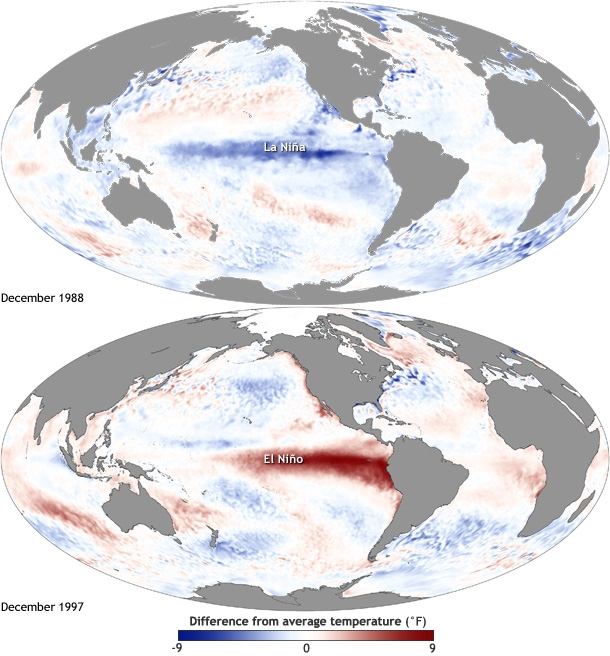
\includegraphics[width=.76\textwidth]{img/enso.jpg}
  \caption[Sea surface temperature during El Ni\~no/La Ni\~na]{
Maps of sea surface temperature (SST) anomaly in the Pacific Ocean during a strong La Ni\~na (top, December 1988) and El Ni\~no (bottom, December 1997). Red is warm and blue is cold. {\bf Note the warmer ocean surface (positive SST anomaly) in the Pacific all the way from the tropics to the Amundsen-Bellingshausen Sea during an El Ni\~no event (in red).} Maps by NOAA Climate.gov, based on data provided by NOAA View (\url{http://www.nnvl.noaa.gov/view/}).
  }
  \label{fig:map-enso}
\end{figure}


\begin{figure}[!ht]
  \centering
  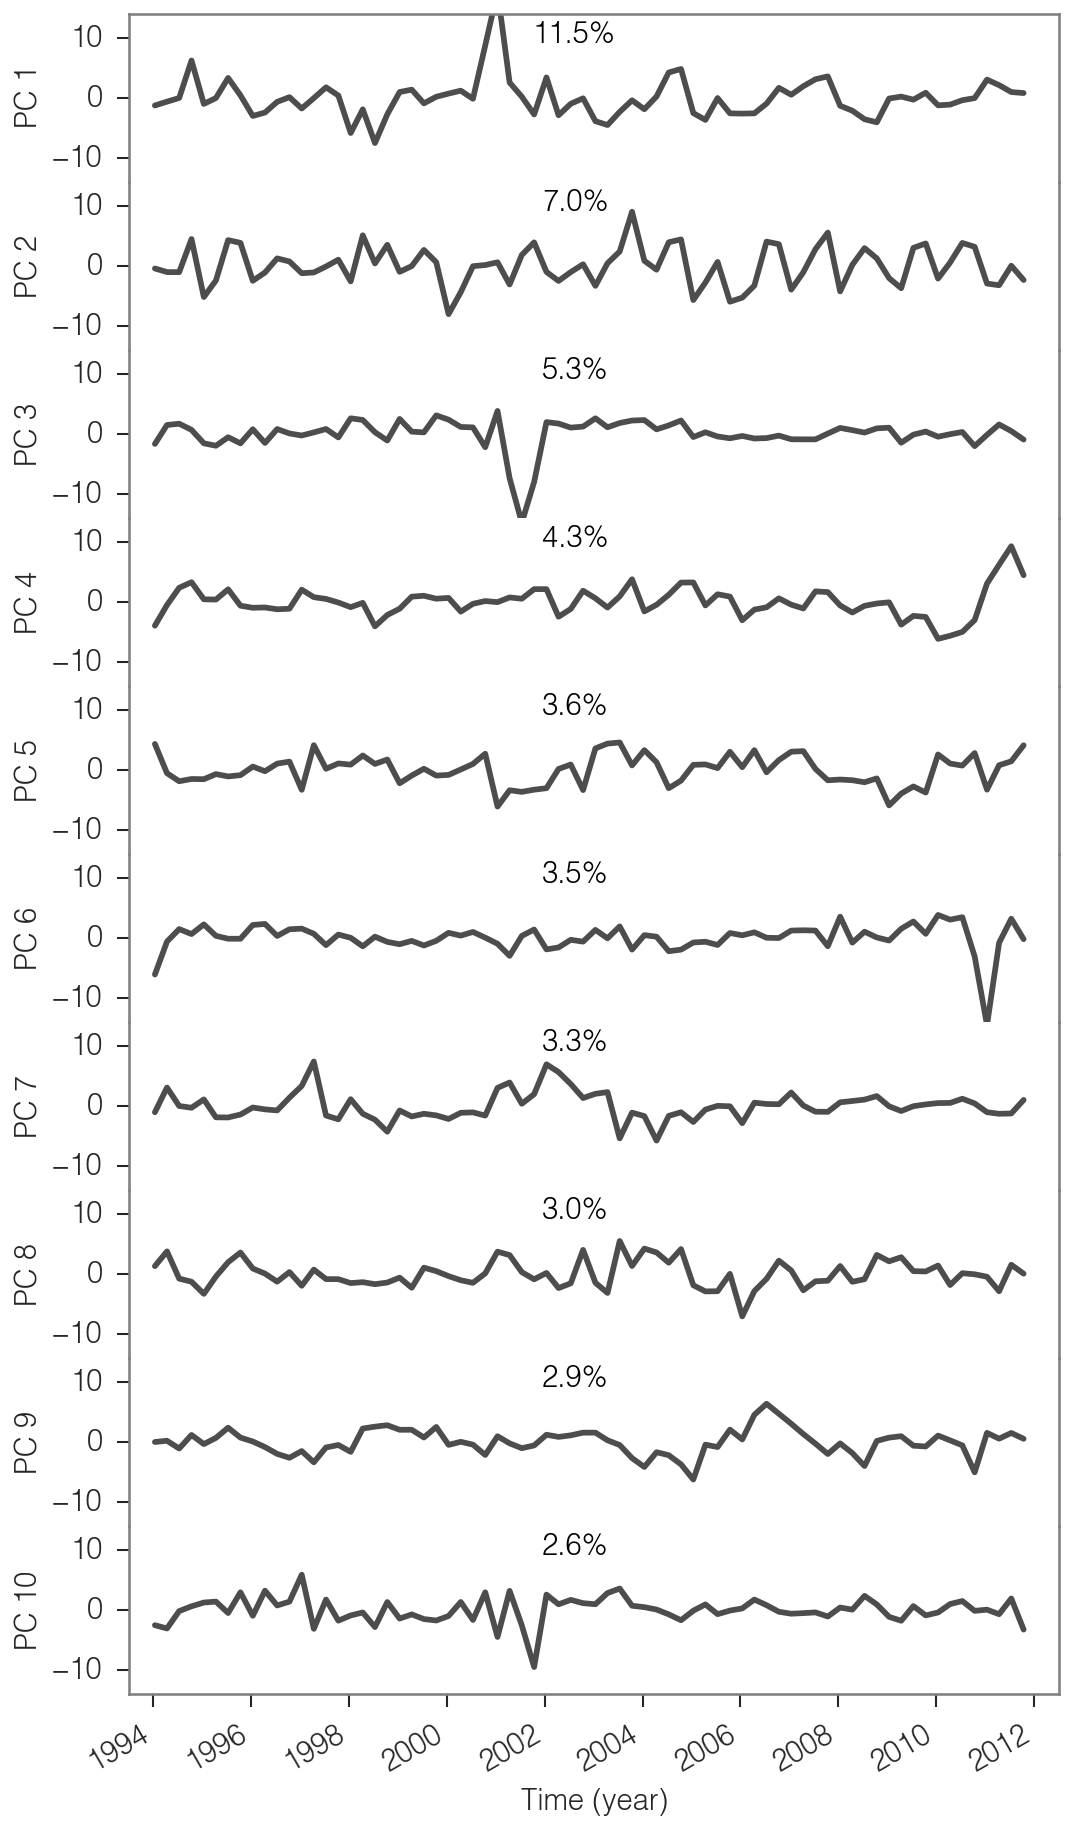
\includegraphics[width=.75\textwidth]{img/mssa_pre_pc_v2.png}
  \caption[Principal components of pre-PCA filtering]{
  Principal components retained after pre-PCA filtering. The ten leading orthogonal components extracted from the original data set (140 time series) by standard PCA. MSSA was then applied to these spatial PCs (i.e., dimensionality was reduced from 140 non-orthogonal series to 10 orthogonal components).
  }
  \label{c4f10}
\end{figure}


\begin{figure}[!ht]
  \centering
  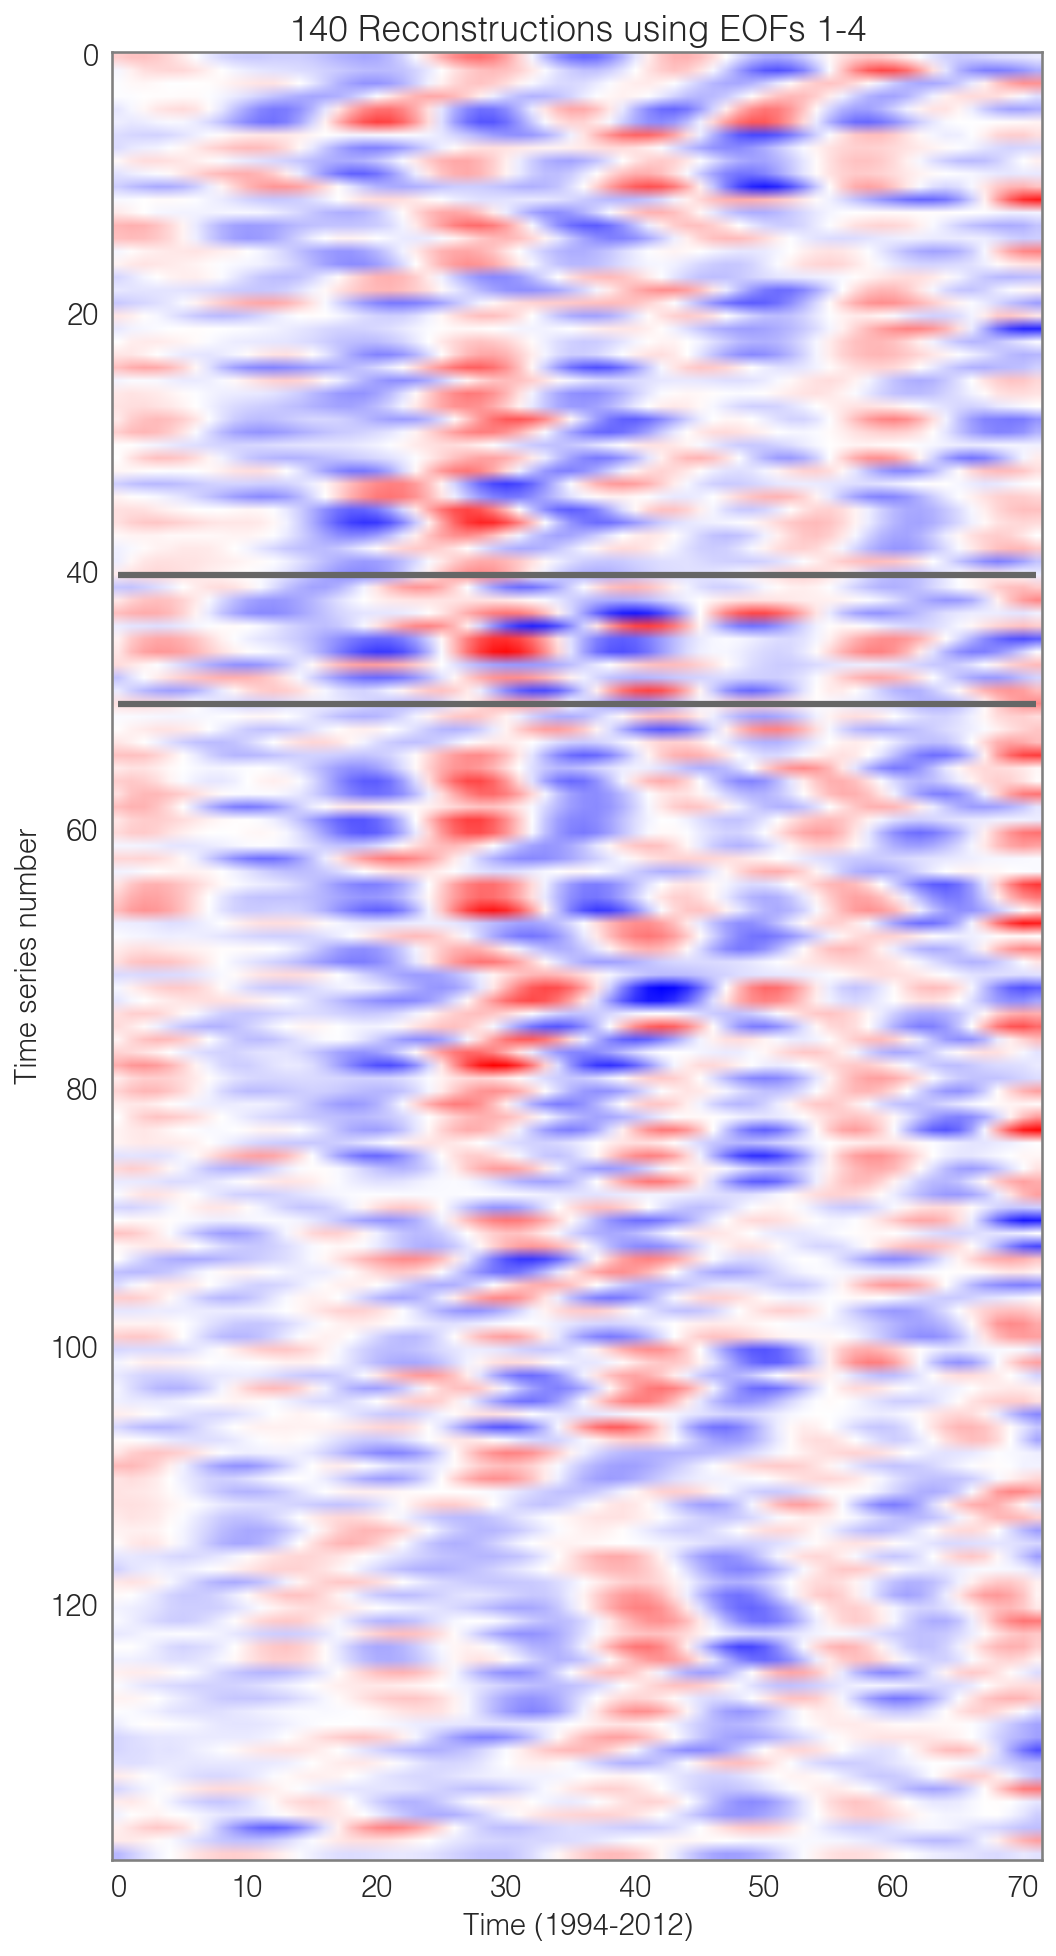
\includegraphics[width=.72\textwidth]{img/amu_rc1234_all.png}
  \caption[Time series reconstruction using EOF 1--4]{
  Time series reconstruction using EOF 1--4. Reconstruction of all 140 time series of ice-shelf height change for the Amundsen region. Red is negative and blue is positive. The gray lines show the ten reconstructions stacked to construct Fig.~\ref{c4f9} (see locations in Fig.~\ref{fig:map-amundsen}).
  }
  \label{fig:rc1234-all}
\end{figure}


\begin{figure}[!ht]
  \centering
  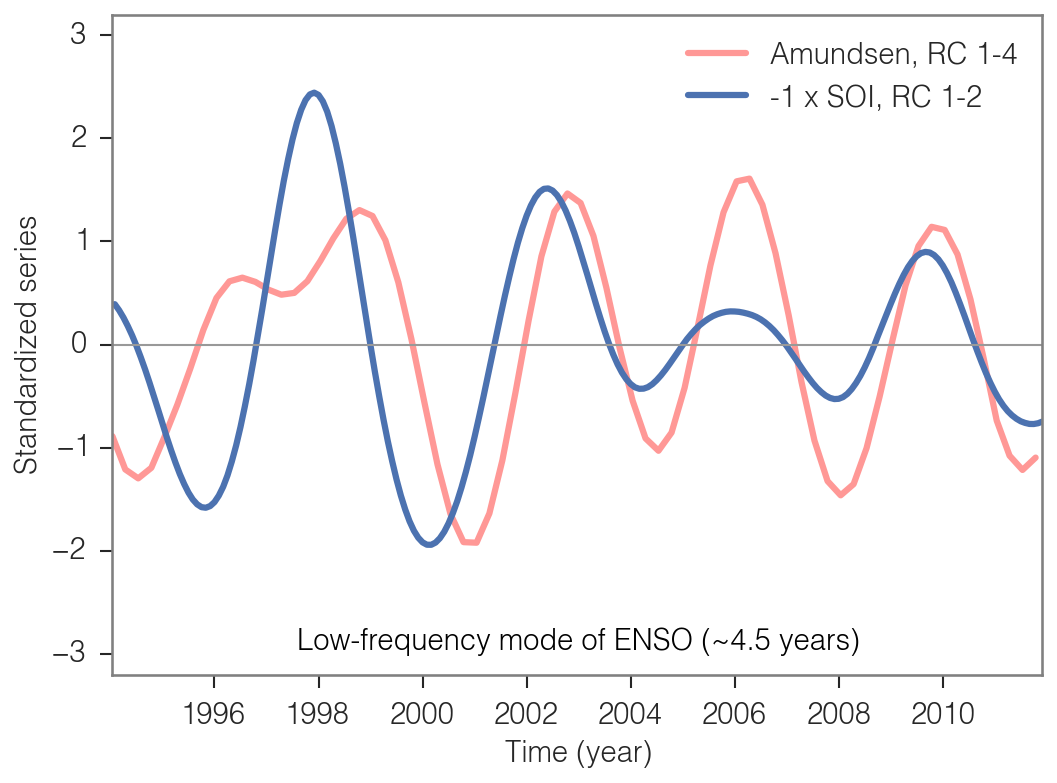
\includegraphics[width=.75\textwidth]{img/amu_soi_modes_all.png}
  \caption[Dominant mode of interannual variability (140 RCs)]{
  Dominant mode of interannual variability (all time series). Reconstruction of the dominant mode of interannual variability for the AS ice-shelf height and the SOI. This is the same as Fig.~\ref{c4f9} but stacking all 140 reconstructions (instead of only 10). Both series show the same dominant frequency of 0.20--0.23 cycle/year (periodicity of $\sim$4.5 years), which corresponds to the low-frequency mode of ENSO.
  }
  \label{c4f12}
\end{figure}


\clearpage
\section*{Acknowledgments}

\noindent
This work was funded by NASA [awards NNX12AN50H 002
(93735A), NNX10AG19G, and NNX13AP60G]. This is ESR
contribution XXX. We thank J. Zwally's Ice Altimetry group
at the NASA Goddard Space Flight Center for distributing their
RA data sets for all satellite radar altimeter missions
(\url{http://icesat4.gsfc.nasa.gov}).

{\sl Chapter 4}, in full, is currently being prepared for submission for publication
of the material. Paolo, Fernando. S.; Fricker, Helen A.; Padman, Laurie. The
dissertation author was the primary investigator and author of this material.
